\documentclass[times, utf8, zavrsni]{fer}
\usepackage{booktabs}
\usepackage[unicode]{hyperref}
\usepackage{algorithm}
\usepackage{algorithmic}
\usepackage{amsmath}
\usepackage{multirow}
\usepackage{subcaption}

\begin{document}

\thesisnumber{6296}

\title{Primjena sustava LCS na klasifikacijske probleme}

\author{Matija Bertović}

\maketitle

% Ispis stranice s napomenom o umetanju izvornika rada. Uklonite naredbu \izvornik ako želite izbaciti tu stranicu.
\izvornik

% Dodavanje zahvale ili prazne stranice. Ako ne želite dodati zahvalu, naredbu ostavite radi prazne stranice.
\zahvala{}

\tableofcontents

\chapter{Uvod}
Ljudi često prilikom zaključivanja i rješavanja problema koriste znanje već stečeno susrećući se s jednostavnijim problemima unutar sličnog područja.
Zašto ne pokušati napraviti sustav temeljen na tehnikama umjetne inteligencije koji ima iste sposobnosti?
U tom slučaju, sustav ne bi svaki problem morao učiti ispočetka, nego bi već sadržavao neko znanje sakupljeno tijekom učenja na manjim problemima.
Na taj bismo način mogli ubrzati vrijeme potrebno za učenje većih problema.
Potrebno je pronaći sustav koji bi mogao imati tu sposobnost.
Sustav bi trebao moći prikupiti i spremiti znanje naučeno na nekom problemu.
Prikupljeno znanje kasnije bi trebalo moći biti iskorišteno prilikom učenja zahtjevnijih problema unutar slične domene.

Sustav koji može omogućiti navedenu funkcionalnost i koji je detaljnije analiziran u ovom radu naziva se sustav LCS \engl{Learning Classifier System}.
Sustav se sastoji od većeg broja pravila, u kojima je sadržano znanje koje on posjeduje.
To znanje kasnije će biti izvučeno i korišteno pri stvaranju novih pravila.

Klasični sustav LCS nema mogućnost iskorištavanja već prikupljenog znanja, nego svaki problem mora učiti od nule, stoga je potrebna promjena koja će to omogućiti.
Sustav je nadograđen, te umjesto klasične ternarne abecede sadrži binarna stabla, slična onima generiranima tehnikama \emph{genetskog programiranja}.

Sustav je testiran na 4 različita problema booleovih funkcija: problem multipleksora, problem većinskog bita, problem parnog pariteta i problem bita prijenosa.
Prilikom implementacije, korištena je ideja Willsonovog sustava XCS temeljenog na preciznosti \citep{2}.

U poglavlju \ref{ch:podr} dan je kratak pregled područja.
Poglavlje \ref{ch:prob} daje detaljniji opis gore navedenih problema koji su rješavani u ovom radu.
Način rada sustava i detaljan opis korištenih algoritama opisan je u poglavlju \ref{ch:algs}.
Rezultati dobiveni primjenom razvijenog sustava opširno su prikazani grafovima i komentirani u poglavlju \ref{ch:res}.
Rad je zaključen i dan je prijedlog budućeg razvoja u poglavlju \ref{ch:zak}.

\chapter{Pregled područja} \label{ch:podr}
Sustavi LCS su sustavi temeljeni na pravilima, koji povezuju \emph{evolucijsko računarstvo} i \emph{strojno učenje} kako bi se što bolje prilagodili rješavanju danog problema.
Sustav je u međudjelovanju s nepoznatom okolinom \engl {environment}, od koje pomoću osjetila \engl{sensors} dobiva ulaz, a preko djelovatelja \engl{effectors} nad njom izvršava određenu akciju \citep{4}.
Sustav se sastoji od skupa određenog broja pravila koja zajedno rješavaju neki problem.
Bitno je naglasiti da poanta učenja nije pronaći jedno pravilo koje na kraju rješava dani problem, nego razviti cijelu populaciju pravila koja ga međusobno rješavaju.
Pravila su najčešće u obliku "AKO \emph{uvjet} ONDA \emph{akcija}".
Uvjet pravila većinom je tvoren od znakova ternarne abecede {0, 1, \#}.
Znakovi 0 i 1 moraju se podudarati s odgovarajućim znakovima ulaza, dok se znak \# podudara s bilo kojim znakom.
Znak \# zovemo simbolom \emph{don't care} \engl{don't care symbol}\footnote{U literaturi se još može naći naziv \emph{wildcard}.} i on omogućava generaliziranje.
Problemi su najčešće takvi da je prostor pretraživanja jako velik i nije moguće doslovno naučiti svaki primjer, nego je potrebna sposobnost generaliziranja.
Prilikom istraživanja novih pravila koriste se tehnike \emph{evolucijskog računarstva} \engl{evolutionary computation}.

Položaj \emph{evolucijskog računarstva} unutar \emph{računarstva} prikazan je slikom \ref{img:racpol}.
\emph{Evolucijsko računarstvo} jedna je od grana \emph{računarstva} iz skupine \emph{mekog računarstva} \engl{soft computing}, zajedno s \emph{neuro-računarstvom} i \emph{neizrazitim računarstvom}.
Ono se bavi algoritmima pretraživanja temeljenima na prirodnoj selekciji.
Cilj je unapređenje početne populacije u kojoj svaka jedinka predstavlja rješenje ili dio rješenja.
Jedinke se trebaju moći vrednovati s obzirom na rješavani problem kako bismo ih mogli uspoređivati.
Za unapređenje populacije jedinki koriste se tehnike selekcije \engl{selection}, križanja \engl{crossover} i mutacije \engl{mutation}.
Selekcija je postupak odabira roditeljskih jedinki iz populacije.
Prilikom odabira roditelja, većinom se u obzir uzima njihova dobrota (jedinke koje imaju veću dobrotu, imaju i veću vjerojatnost odabira za roditeljsku jedinku).
Nakon odabira roditelja, dolazi do njihovog križanja te tako nastaju potomci \engl{offspring}.
Križanje je kombiniranje genetskog materijala roditelja čime se stvaraju potomci koji dio svog genetskog materijala naslijede od jednog, a dio od drugog roditelja.
Nakon križanja, javlja se mutacija gena potomaka.
Svaki gen ima određenu vjerojatnost mutacije.
Mutacijom gen može promijeniti trenutnu vrijednost u neku novu koja ovisi o trenutnoj ili se može generirati potpuno novi gen.
Više informacija o \emph{evolucijskom računarstvu} i \emph{genetskim algoritmima} čitatelj može pronaći u \citep{6}.
\begin{figure}[!h]
    \centering
    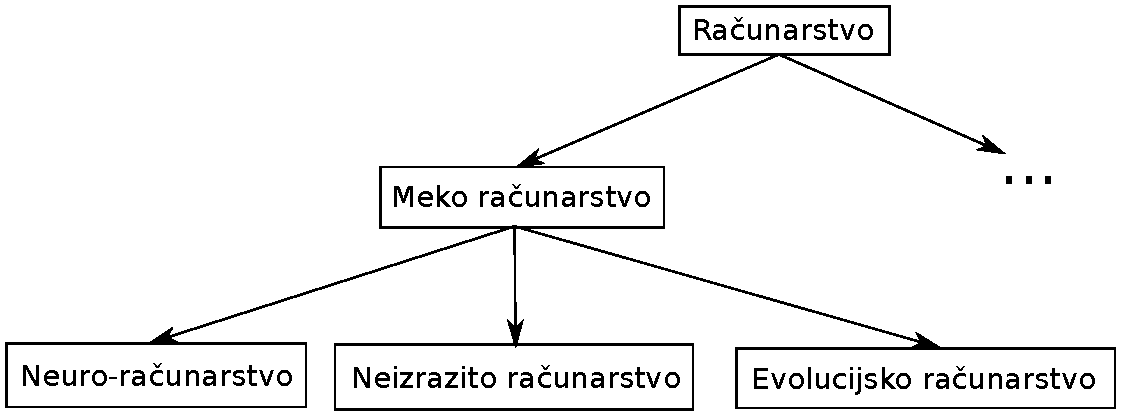
\includegraphics[width=\textwidth]{img/racpol.pdf}
    \caption{Položaj \emph{evolucijskog računarstva} unutar \emph{računarstva}.}
    \label{img:racpol}
\end{figure}

Prilikom rada sustava LCS, pravila djeluju zajedno, ali neka su \emph{bolja} i imaju veću sposobnost generaliziranja od drugih.
Kako bi razlikovali različita pravila i u kojoj mjeri ona utječu na konačni ishod sustava, pravilima se dodjeljuju razni parametri.
Ažuriranje tih parametara obavlja se tehnikama \emph{podržanog učenja} \engl{reinforcement learning}, koje usmjerava potragu za boljim pravilima \citep{3}.

\begin{figure}[!h]
    \centering
    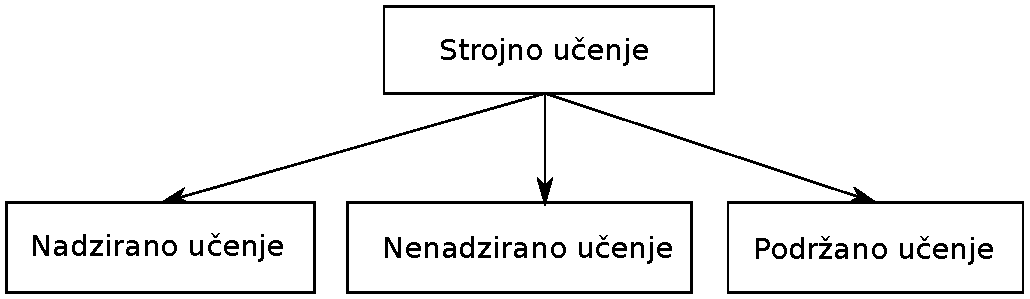
\includegraphics[width=\textwidth]{img/ml.pdf}
    \caption{Položaj \emph{podržanog učenja} unutar \emph{strojnog učenja}.}
    \label{img:repol}
\end{figure}
\emph{Podržano učenje} grana je \emph{strojnog učenja} \engl{machine learning} zajedno za \emph{nadziranim} \engl{supervised} i \emph{nenadziranim učenjem} \engl{unsupervised learning}, kao što je prikazano na slici \ref{img:repol}.
\emph{Podržano učenje} temeljeno je na pokušajima, nakon kojih sustav dobije određenu brojčanu nagradu.
Cilj sustava temeljenog na podržanom učenju je maksimizirati nagradu koju sustav dobije izvršavanjem neke akcije.
U ovisnosti o dobivenoj nagradi, sustav podešava svoje parametre kako bi s vremenom dobivao sve veću i veću nagradu.
Značajka \emph{podržanog učenja} je da sustav ne uči na poznatim točnim ishodima, nego on sam odabire svoju akciju na temelju koje dobiva određenu brojčanu nagradu.
Na taj način je sustav primoran učiti samo iz svog prethodnog iskustva.
Detaljniju analizu \emph{podržanog učenja} čitatelj može pronaći u \citep{7}.

Dva glavna pristupa u implementaciji sustava LCS su \emph{michiganski stil} \engl{Michigan-Style} i \emph{pittsburgski stil} \emph{Pittsburgh-Style}.
\emph{Pittsburgski stil} sustava LCS sadrži skup jedinki od kojih je svaka moguće konačno rješenje sustava.
Jedna jedinka je cijeli skup pravila, što znači da je karakteristika \emph{pittsburgskog stila} da sadrži više neovisnih skupova pravila.
Iako pravila moraju biti jednake duljine, svaki skup pravila može sadržavati različit broj pravila.
\emph{Genetski algoritam} pokreće se nad cijelim skupom jedinki, odnosno na skupom skupova pravila.

U okviru ovog rada obrađen je \emph{michiganski stil} sustava LCS.
\emph{Michiganski stil} sustava LCS okarakteriziran je jednim skupom pravila.
Svako pravilo predstavlja jednu jedinku.
Jedinka u \emph{michiganskom stilu} sustava LCS ne predstavlja konačno rješenje sustava, nego je konačno rješenje cijeli skup jedinki, odnosno jedinke djeluju zajedno pri rješavanju problema.
\emph{Michiganski stil} sustava LCS prvi je formalizirao John Holland 1976. godine, a u suradnji s Judith Reitman 1978. dao njegovu implementaciju.
S obzirom na složenost originalnog LCS sustava, malo jednostavniju i razumljiviju inačicu dao je Stewart W. Wilson pod nazivom ZCS \engl{"zeroth-level" classifier system}.
Nakon toga, Wilson je uveo još jednu inačicu suatava LCS pod nazivom XCS, u kojemu je promijenio način na koji se računa $dobrota$ pojedinih pravila.
U sklopu ovog rada obrađen je sustav XCS, koji je detaljno objašnjen u poglavljima koja slijede, a za detaljniji opis prvotnog sustava LCS i sustava ZCS čitatelj se upućuje na \citep{3}.

\begin{figure}[h]
    \centering
    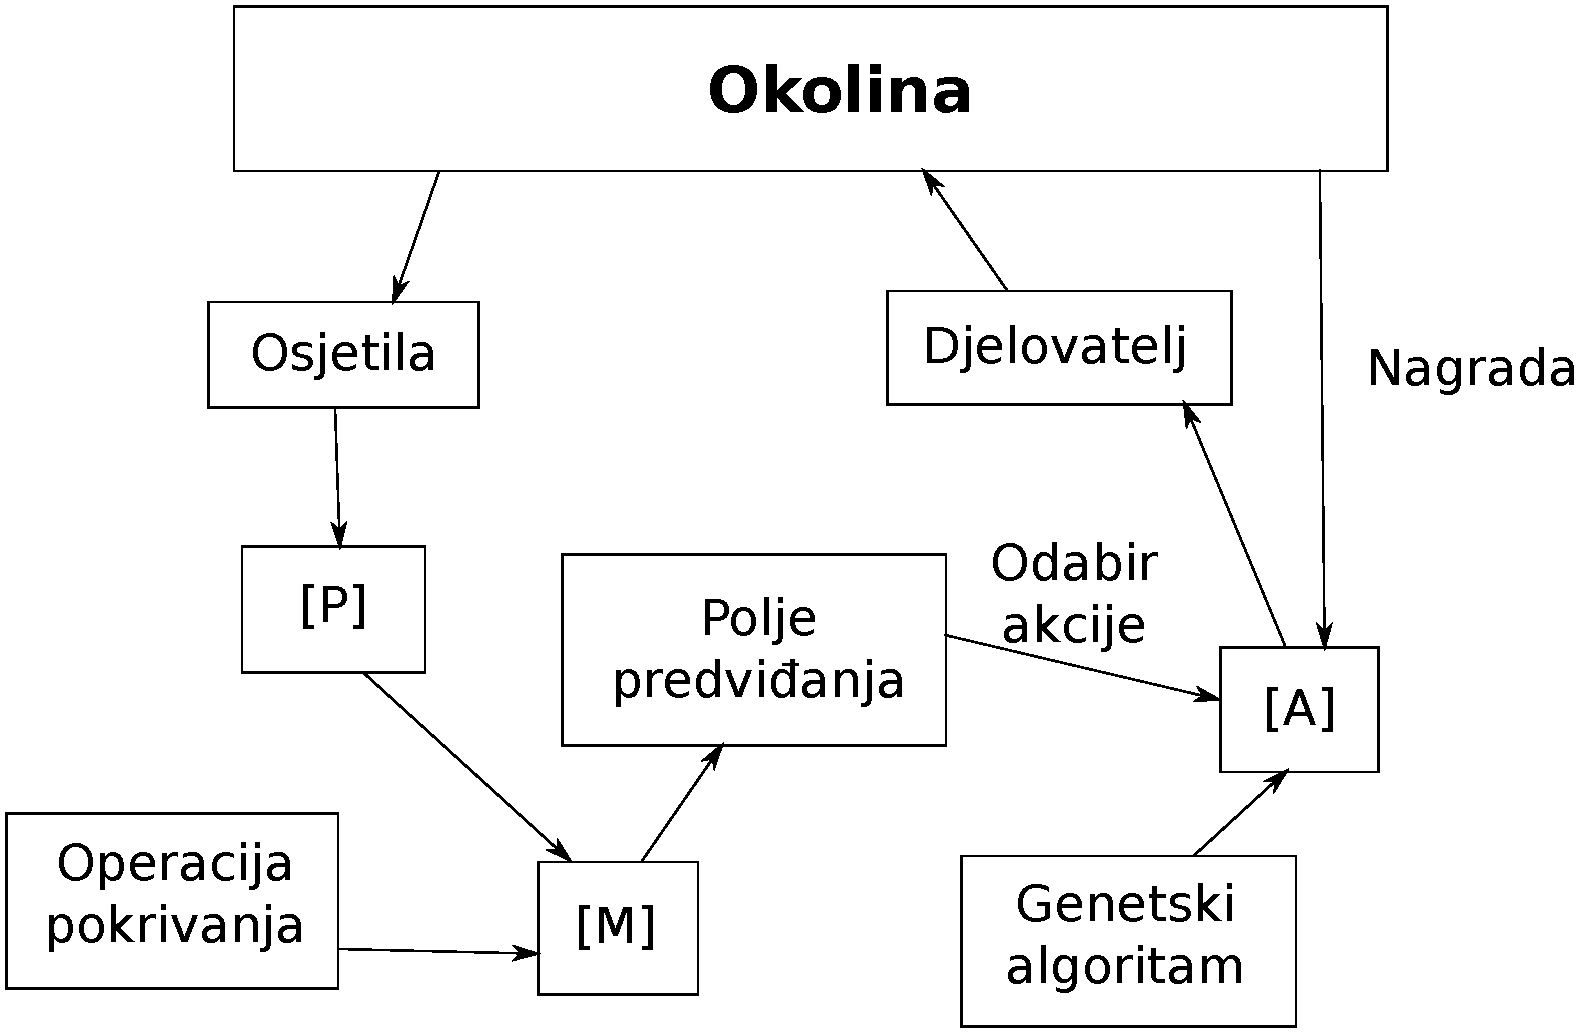
\includegraphics[width=\textwidth]{img/xcs.pdf}
    \caption{Ilustracija sustava XCS.}
    \label{img:xcs}
\end{figure}
Ilustracija međudjelovanja komponenti sustava XCS prikazana je na slici \ref{img:xcs}.
Prilikom rada sustava izmjenjuju se načini rada \emph{istraži} \engl{explore} i \emph{iskoristi} \engl{exploit}.
U načinu rada \emph{istraži}, sustav se prilagođava zadanom problemu mijenjanjem svoje konfiguracije, a u načinu rada \emph{iskoristi} sustav se ne mijenja, nego se na temelju trenutne konfiguracije predviđa akcija koju treba izvršiti.

Prilikom načina rada \emph{istraži} sustav najprije od nepoznate okoline preko osjetila dobije ulazni podatak.
Po primitku podatka, skeniraju se sva pravila unutar populacije pravila [\emph{P}].
Od svih pravila iz [\emph{P}], od onih koja odgovaraju dobivenom ulaznom podatku tvori se podudarni skup \engl{match set} [\emph{M}].
Nakon formiranja podudarnog skupa [\emph{M}], u slučaju da on ne sadrži barem jedno pravilo za svaku moguću akciju, pokreće se operacija pokrivanja \engl{covering operation}.
Operacija pokrivanja generira proizvoljno pravilo koje odgovara zadanom ulazu i traženoj akciji te ga dodaje u populaciju.
Nakon što je formiran konačni podudarni skup, tvori se polje predviđanja \engl{prediction array}.
Polje predviđanja za svaku moguću akciju sadrži podatak o tome kolika se prosječna nagrada očekuje izvršavanjem te akcije.
Na temelju polja predviđanja izabire se konačna akcija koju će sustav izvršiti za dani ulazni podatak.
Odabirom konačne akcije, skenira se podudarni skup i tvori se akcijski skup \engl {action set} [\emph{A}].
Akcijski skup sastoji se od svih pravila sadržanih u podudarnom skupu koja zagovaraju odabranu konačnu akciju.
Po formiranju akcijskog skupa, nad okolinom se, preko djelovatelja, izvršava odabrana akcija.
Nakon toga, okolina u ovisnosti o izvršenoj akciji sustavu dodjeljuje određenu numeričku nagradu \engl {reward}.
Što je sustav izvršio bolju akciju u ovisnosti o ulaznom podatku, to je nagrada veća i obrnuto.
Cilj sustava je maksimizirati nagradu koju dobije od okoline.
Na temelju dobivene nagrade, sustav ažurira određene parametre svih pravila unutar akcijskog skupa, u svrhu povećanja buduće nagrade.
Nakon ažuriranja parametara, ako je zadovoljen određeni uvjet, uključuje se istraživačka komponenta koja primjenom \emph{genetskog algoritma} istražuje nova pravila.
Operacija istraživanja novih pravila djeluje isključivo nad akcijskim skupom.

Prilikom načina rada \emph{iskoristi} isključuju se sve istraživačke komponente.
Sustav preko osjetila od okoline dobije ulazni podatak.
Po primitku podatka tvori se podudarni skup sa svim pravilima iz populacije koja odgovaraju dobivenom ulaznom podatku.
Nakon toga, tvori se polje predviđanja, kao i u načinu rada \emph{istraži}.
Sada se na temelju polja predviđanja izabire ona akcija čijim izvršavanjem se očekuje najveća nagrada okoline.
Trenutna iteracija ovdje završava te se čeka sljedeći podatak na ulazu.

Ovaj cijeli postupak detaljno je opisan u poglavlju \ref{ch:algs} gdje su točno opisani i korišteni pripadni algoritmi.

\chapter{Opis problema} \label{ch:prob}
Problemi testirani u ovom radu su:
\begin{enumerate}
    \item multipleksor \engl{multiplexer},
    \item paritetni bit \engl{parity},
    \item najzastupljeniji bit \engl{majority-on},
    \item bit prijenosa binarnog zbrajala \engl{carry}.
\end{enumerate}

Najviše pažnje posvećeno je rješavanju multipleksora.
Na slici \ref{img:mux} prikazan je multipleksor 4/1.
Multipleksor 4/1 ima 2 upravljačka bita i 4 ulazna bita te jedan izlazni bit.
Upravljački bitovi određuju točno jedan ulazni bit koji se dalje prosljeđuje na izlaz, kako je prikazano u tablici \ref{tbl:mux}.
\begin{figure}[h]
    \centering
    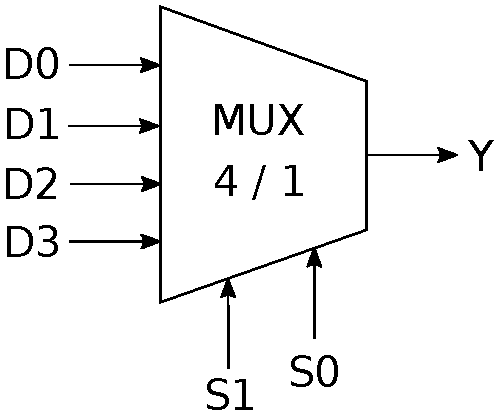
\includegraphics[width=5cm]{img/mux.pdf}
    \caption{Multipleksor 4/1.}
    \label{img:mux}
\end{figure}
Općenito, multipleksor koji ima $k$ upravljačkih bitova funkcionira na isti način.
$k$ upravljačkih bitova može adresirati $2^{k}$ ulaznih bitova, stoga je multipleksor s $k$ upravljačkih bitova funkcija od $k + 2^{k}$ varijabli.
Izlaz iz multipleksora je uvijek točno 1 bit, koji ima vrijednost 0 ili 1.
\begin{figure}[h]
    \centering
    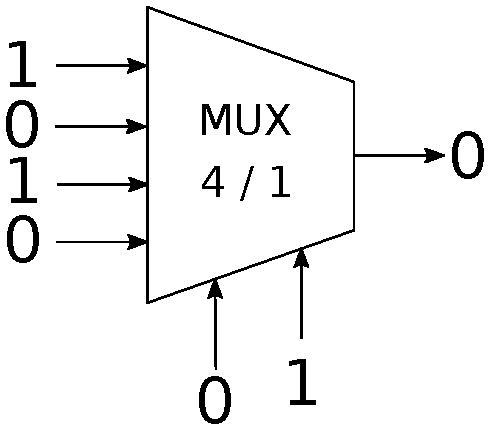
\includegraphics[width=5cm]{img/muxex.pdf}
    \caption{Konkretan primjer 4/1 multipleksora.}
    \label{img:muxex}
\end{figure}
Na slici \ref{img:muxex} dan je konkretan primjer 4/1 multipleksora.
Upravljači bitovi ovdje su 01, a ulazni 1010.
Upravljački bitovi adresiraju drugi ulaz u multipleksor, stoga se on propušta na izlaz.
Na izlazu vidimo vrijednost 0, koja odgovara drugom ulazu.
U implementaciji, ovaj primjer bi na ulaz bio dan kao niz bitova 011010.
Ulaz se prvo sastoji od upravljačih bitova, a zatim ulaznih.
Očekivani izlaz bi u ovom slučaju bio 0.
\begin{table}[!htb]
    \caption{Opis rada multipleksora 4/1.}
    \label{tbl:mux}
    \centering
    \begin{tabular}{c | c | c}
        $S_{1}$ & $S_{0}$ & $Y$     \\ \hline
              0 &       0 & $D_{0}$ \\
              0 &       1 & $D_{1}$ \\
              1 &       0 & $D_{2}$ \\
              1 &       1 & $D_{3}$ \\
    \end{tabular}
\end{table}

Problem paritetnog bita svodi se na ispitivanje broja pojavljivanja bita 1 unutar ulaza.
Sklop za određivanje paritetnog bita za parni paritet na ulaz prima $n$-bitni binarni broj te vraća broj s ulaza proširen jednim dodatnim bitom, koji osigurava da je broj pojavljivanja bita 1 paran, odnosno osigurava parni paritet.
Dodani bit naziva se paritetni bit.
Ako je broj pojavljivanja bita 1 na ulazu paran, broj se treba proširiti bitom 0, a u suprotnom bitom 1.
Primjer jednog takvog sklopa koji radi za 6-bitne binarne brojeve prikazan je na slici \ref{img:parex}. Prikazani sklop na ulaz prima 6-bitni binarni broj 011010.
Ulazni podatak ima neparan broj (3) jedinica, dakle treba ga proširiti bitom 1.
Sklop na izlazu vraća 7-bitni binarni broj \textbf{1}011010 koji ima paran broj (4) jedinica.
Prilikom rješavanja ovog problema, razvijeni sustav određuje samo prikazani paritetni bit za parni paritet, a ne cijeli novi $n + 1$-bitni broj.
\begin{figure}[h]
    \centering
    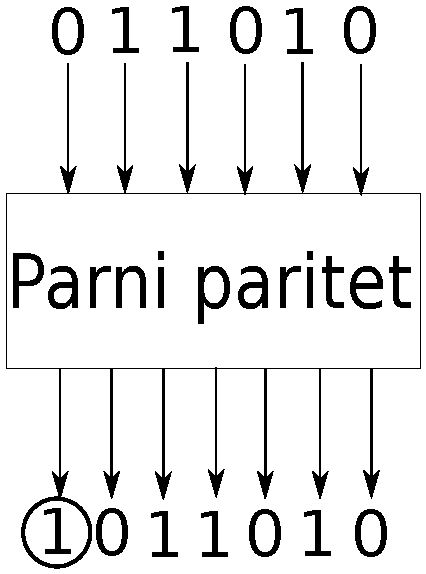
\includegraphics[width=5cm]{img/parity.pdf}
    \caption{Primjer sklopa za određivanje paritetnog bita na 6-bitnom binarnom broju.}
    \label{img:parex}
\end{figure}

Prilikom problema najzastupljenijeg bita, ispituje se frekvencija pojavljivanja pojedinih bitova.
Sklop za određivanje najzastupljenijeg bita na ulaz prima $n$-bitni binarni broj i na izlaz vraća samo jedan bit, bit koji se najviše puta pojavio u ulaznom binarnom broju.
Primjer jednog takvog sklopa koji na ulaz prima 7-bitni binarni broj prikazan je na slici \ref{img:majex}.
Ulaz u sklop je binarni broj 1011010.
Ulazni broj ima 4 bita 1 i 3 bita 0.
S obzirom da je broj pojavljivanja bita 1 veći od broja pojavljivanja bita 0, na izlaz se vraća bit 1.
Prilikom rješavanja problema najzastupljenijeg bita, ulazni brojevi uvijek su neparne duljine, kako bi se izbjeglo pojavljivanje jednakog broja bitova 0 i bitova 1.
\begin{figure}[h]
    \centering
    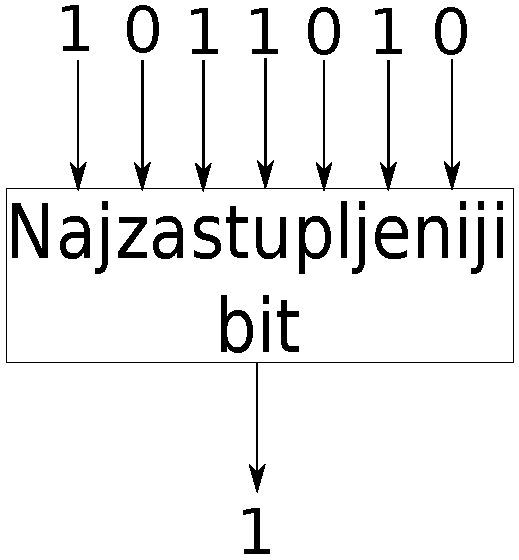
\includegraphics[width=5cm]{img/majority.pdf}
    \caption{Primjer sklopa za određivanje najzastupljenijeg bita na 7-bitnom binarnom broju.}
    \label{img:majex}
\end{figure}

Na slici \ref{img:caex} dan je primjer rada 7-bitnog binarnog zbrajala.
Višebitno binarno zbrajalo na ulaze prima bitove oba pribrojnika.
Bitovi pribrojnika šalju se u grupama prema težini.
Iz slike je vidljivo da se 3-bitno binarno zbrajalo sastoji od 3 komponente.
Općenito, $n$-bitno binarno zbrajalo sastoji se od $n$ komponenti.
Komponenta označena slovom $H$ je poluzbrajalo \engl{half-adder}.
Poluzbrajalo na ulaze prima dva bita, na jedan izlaz vraća njihov zbroj (označen strelicom prema dolje), a na drugi izlaz vraća bit prijenosa (označen strelicom prema lijevo).
Komponente označene slovima $FA$ su potpuna zbrajala \engl{full-adder}.
Potpuno zbrajalo na ulaze prima 3 bita, a kao i poluzbrajalo, na izlaze vraća zbroj tih bitova i bit prijenosa.
U prikazanom primjeru, prvi binarni broj je 110, a drugi binarni broj 011.
Rezultat zbrajanja je binarni broj 001, a konačni bit prijenosa, koji predstavlja izlaz iz 3-bitnog zbrajala je 1.
U implementaciji je ulaz u $n$-bitno binarno zbrajalo prikazan redom bitovima prvog pa drugog pribrojnika i on je veličine $2n$, a izlaz je konačni bit prijenosa.
Testirajući ovaj primjer, podatak dobiven iz okoline bio bi 110011, a očekivani izlaz bio bi 1.
Ulazni podatak uvijek će biti parne duljine $2n$, kako bi se on mogao interpretirati kao 2 $n$-bitna binarna broja.
\begin{figure}[!h]
    \centering
    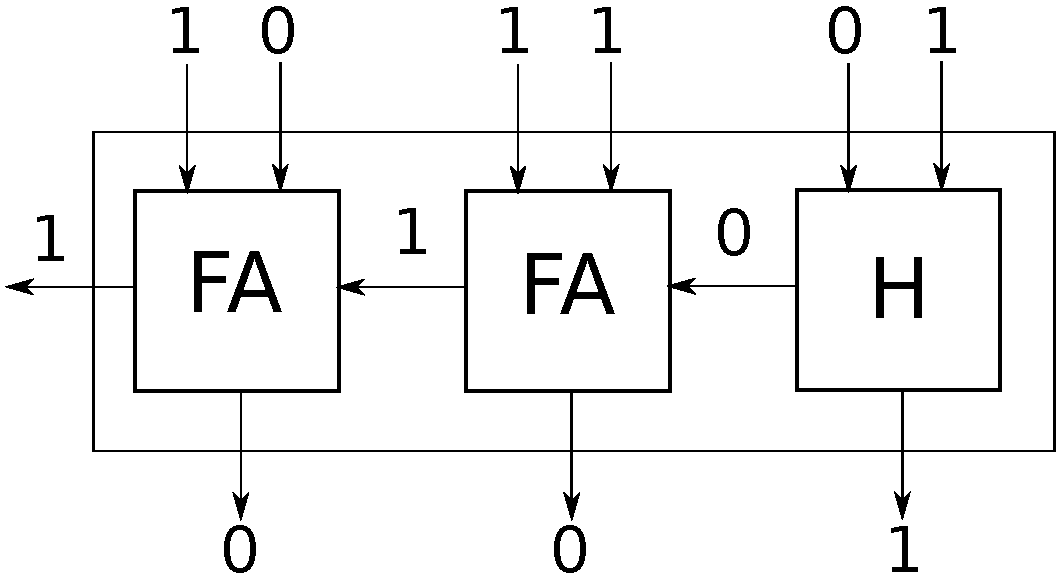
\includegraphics[width=13cm]{img/fa.pdf}
    \caption{Primjer višebitnog binarnog zbrajala za zbrajanje 3-bitnih binarnih brojeva.}
    \label{img:caex}
\end{figure}

\chapter{Opis algoritama} \label{ch:algs}
U sklopu razrade ovog sustava, potrebno je ostvariti iskorištavanje znanja već naučenog na jednostavnijim problemima.
Klasični bitovi uvjeta u ranije opisanim pravilima nam to onemogućavaju.
Iz tog razloga, svaki bit uvjeta zamijenjen je programskim isječkom, koji ovisno o ulazu, vraća 0 ili 1.
Takav sustav XCS, koji koristi programske isječke umjesto uvjetnih bitova, naziva se XCSCFC\footnote{Kratica dolazi od engl. \emph{XCS with code-fragment conditions}.}.
Na taj način, prilikom stvaranja novih pravila, ona mogu sadržavati programske isječke izvučene iz pravila koja su rješavala jednostavniji problem u istoj domeni.
Prilikom preuzimanja programskih isječaka, u obzir dolaze samo precizna i iskusna pravila čija dobrota \engl{fitness} je veća od prosječne unutar te populacije pravila \citep{4}.

U ovom radu, isječci koda modelirani su binarnim stablima dubine do najviše 2, što znači da je moguće imati najviše 7 čvorova.
Skup funkcija koje čvorovi mogu obavljati je $\{AND, OR, NAND, NOR, NOT\}$.
U primjerima, te su funkcije redom označene s $\&, |, d, r, \sim$.
Skup mogućih završnih (terminalnih) čvorova pojedinog binarnog stabla je $\{D_{0}, D_{1}, ..., D_{n - 1}\}$, gdje \emph{n} predstavlja duljinu ulaza dobivenog od okoline.
Svaki završni čvor predstavlja točno jedan bit ulaza.
Svaki programski isječak na ulaz dobiva cijeli ulaz dobiven od okoline, a na izlazu vraća rezultat operacija koje se nalaze u čvorovima stabla.
Na slici \ref{tree} prikazan je primjer jednog takvog binarnog stabla koje vraća rezultat operacije $D_{3}D_{1}dD_{0}D_{1}|\&$.
Operacija je zbog jednostavnosti prikazana u \emph{postfiks} obliku.
Iz slike je vidljivo da se u binarnom stablu ne moraju pojavljivati svi bitovi ulaza, a također i da se pojedini bitovi mogu pojavljivati više puta.
\begin{figure}[h]
    \centering
    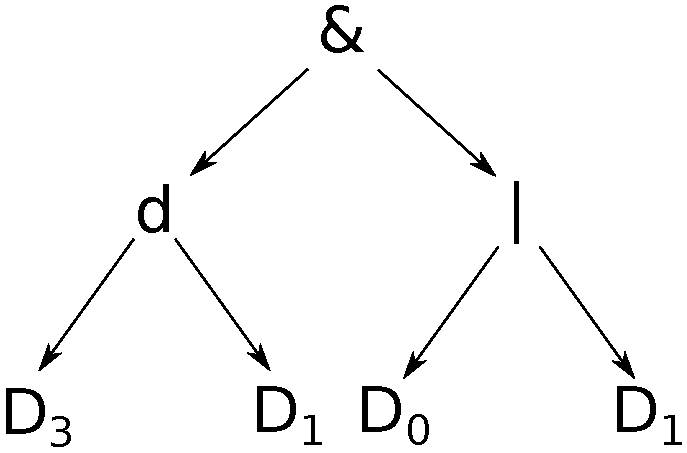
\includegraphics[width=8cm]{img/tree.pdf}
    \caption{Primjer programskog isječka prikazanog binarnim stablom.}
    \label{tree}
\end{figure}

Potreban je i programski isječak koji označava simbol \emph{don't care}, a koji za svaki niz bitova koje dobije na ulazu, na izlazu vraća 1.
On je prikazan na slici \ref{dnc} i označava operaciju $D_{0}D_{0}\sim|$, a preuzet je iz \citep{4}.
\begin{figure}[h]
    \centering
    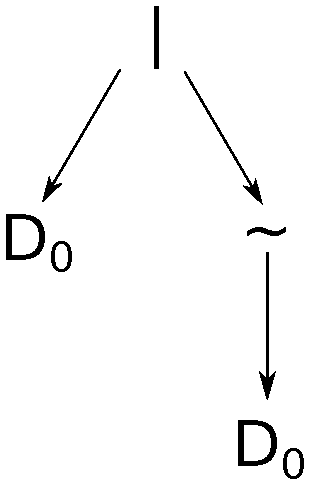
\includegraphics[height=6cm]{img/dnc.pdf}
    \caption{Isječak koda korišten kao simbol \emph{don't care}.}
    \label{dnc}
\end{figure}

Prije detaljnog objašnjenja korištenih algoritama, potrebno je naglasiti da su u implementaciji korišteni makroklasifikatori \engl{macroclassifiers} \citep{2}.
Makroklasifikatori su pravila koji imaju dodatan parametar brojnosti \engl{numerosity}.
Razlog korištenju makroklasifikatora je bolja vremenska i prostorna složenost sustava.
Naime, pravila koja imaju jednaki uvjet i akciju sadržana su u istom pravilu, ali je njegova brojnost u tom slučaju veća od 1.
Brojnost pravila $cl$ sadržana je u varijabli $cl.n$.
Ako u populaciji postoji $n$ pravila koji imaju jednak uvjet i akciju, to je zapisano u jednom pravilu čija je brojnost u tom slučaju postavljena na $n$.
Kod korištenja makroklasifikatora, prilikom svih izračuna potrebno je u obzir uzeti i parametar brojnosti.

U načinu rada \emph{istraži}, na početku se od okoline dobije ulazni podatak $s$.
U ovisnosti o $s$, formira se \emph{podudarni skup} [\emph{M}].
[\emph{M}] se sastoji od svih pravila iz populacije [\emph{P}] koji odgovaraju ulazu $s$.

Za pravilo $cl$\footnote{Kratica dolazi od engl. \emph{classifier}. Naime, u ovom je slučaju cijeli sustav jedan klasifikator koji raspoređuje podatke u razrede, ali i za svako pravilo se može reći da je jedan \emph{mali} klasifikator. S obzirom da samo pravilo pojedinačno ne radi ispravnu klasifikaciju, ovdje ga ispravine zovemo \emph{pravilo}, a ne \emph{klasifikator}.} kažemo da odgovara ulazu $s$, ako svaki programski isječak za zadani ulaz $s$ na izlazu daje 1.
S obzirom da svaki programski isječak unutar uvjeta pravila na ulaz dobiva cijeli $s$, poredak programskih isječaka unutar pravila uopće nije bitan.
Algoritam \ref{match} prikazuje postupak evaluacije pravila $cl$ u odnosu na ulaz $s$.
Pri tome $cf$ označava \emph{i}-ti programski isječak unutar zadanog pravila $cl$, a $val$ rezultat programskog isječka $cf$ s obzirom na zadani ulaz $s$.
$n$ je duljina uvjeta unutar pravila, odnosno broj programskih isječaka koji se nalaze u pravilu.
$cl.cond$ je polje svih programskih isječaka.
Algoritam vraća vrijednost $true$ ako svaki programski isječak za zadani ulaz $s$ vraća vrijednost 1, a $false$ inače.

\begin{algorithm}
    \caption{Evaluiranje pravila $cl$ u odnosu na ulaz $s$}
    \label{match}
    \begin{algorithmic}
        \STATE{\textbf{Ulaz:} $cl$ -- pravilo, $s$ -- stanje okoline.}
        \STATE{\textbf{Izlaz:} odgovara li pravilo $cl$ stanju $s$}
        \FOR{($i := 0; i < n; i := i + 1$)}
        \STATE{$cf := cl.cond[i]$}
        \STATE{$val := evaluiraj(cf, s)$}
        \IF{$val \neq 1$}
        \RETURN{$false$}
        \ENDIF
        \ENDFOR
        \RETURN{$true$}
    \end{algorithmic}
\end{algorithm}

Primjer izgleda jednog opisanog pravila prikazan je na slici \ref{img:clex}.
Vidimo da zadano pravilo ima 3 uvjetna bita i jedan simbol \emph{don't care}.
Prikazano pravilo određuje akciju 1.
Pretpostavimo da iz okoline dobijemo ulaz 011.
Ulaz se za zadano pravilo evaluira za svaki uvjetni bit pravila.
Da bi se ulaz i pravilo mogli podudarati, svaki programski isječak uvjeta pravila mora vratiti 1, u suprotnom se ulaz i pravilo ne podudaraju.
Prvi programski isječak izvodi funkciju $D_{0}D_{0}\sim|$, što bi se na danom primjeru pretvorilo u $00\sim|$, a to se evaluira u 1.
Ovo je ujedno i simbol \emph{don't care} koji se uvijek evaluira u 1.
Drugi programski isječak izvodi funkciju $D_{2}D_{1}D_{0}\&d$, što se pretvara u $110\&d$, a evaluira u 1.
Posljednji programski isječak izvodi funkciju $D_{2}$, koja se pretvara u $1$ i evaluira u 1.
Pokazano je da se sva tri programska isječka za ovaj ulaz evaluiraju u 1, stoga bismo mogli reći da se ovo pravilo i ulaz podudaraju.
\begin{figure}[h]
    \centering
    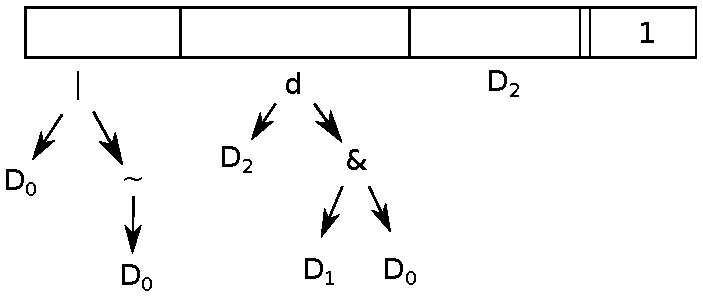
\includegraphics[height=6cm]{img/clex.pdf}
    \caption{Primjer izgleda jednog konkretnog pravila s 3 uvjetna bita.}
    \label{img:clex}
\end{figure}

Nakon formiranja [\emph{M}], provjerava se sadrži li [\emph{M}] sve moguće akcije $a$.
U slučaju da za neku akciju ne postoji pripadno pravilo, pokreće se operacija pokrivanja \engl{covering operation}, prikazana algoritmom \ref{cover}.
U operaciji pokrivanja stvara se novo pravilo čiji je svaki programski isječak simbol \emph{don't care} s vjerojatnošću $P_{don'tCare}$, a s vjerojatnošću $1 - P_{don'tCare}$ proizvoljno generirani programski isječak, koji s obzirom na stanje $s$ mora vraćati 1.
U prikazanom algoritmu, $cl.action$ sadrži akciju koju zagovara pravilo $cl$.
Operacija pokrivanja pokreće se za svaku akciju koja nedostaje u [\emph{M}], a novo pravilo se dodaje u [\emph{P}] i [\emph{M}].

\begin{algorithm}
    \caption{Operacija pokrivanja}
    \label{cover}
    \begin{algorithmic}
        \STATE{\textbf{Ulaz:} $s$ -- ulaz dobiven iz okoline, $a$ -- akcija koju se pokriva.}
        \STATE{\textbf{Izlaz:} Generirano novo pravilo $cl$}
        \STATE{$cl$ := inicijaliziraj novo pravilo}
        \FOR{($i := 0; i < n; i := i + 1$)}
        \STATE{$r$ := proizvoljan decimalni broj iz intervala [0, 1)}
        \IF{$r < P_{don'tCare}$}
        \STATE{$cl.cond[i]$ := \emph{don't care} simbol}
        \ELSE
        \REPEAT
        \STATE{$cf$ := generiraj proizvoljni programski isječak}
        \STATE{$val := evaluiraj(cf, s)$}
        \UNTIL{$val \neq 1$}
        \STATE{$cl.cond[i] := cf$}
        \ENDIF
        \ENDFOR
        \STATE{$cl.action := a$}
        \RETURN{$cl$}
    \end{algorithmic}
\end{algorithm}

Nakon svakog novog dodavanja pravila u [\emph{P}], pokreće se operacija brisanja \citep{1}.
S obzirom da je potrebno zadržati maksimalnu veličinu populacije $N$, ako je trenutna veličina populacije veća od $N$, izabiru se pravila koja je potrebno izbrisati.
Operacija brisanja prikazana je algoritmom \ref{del}.
Pravilo se za brisanje odabire \emph{Roulette-Wheel} postupkom, na temelju glasova koje daje svako pravilo.
\begin{algorithm}
    \caption{Operacija brisanja}
    \label{del}
    \begin{algorithmic}
        \STATE{\textbf{Ulaz:} $[P]$ -- populacija.}
        \STATE{\textbf{Izlaz:} -}
        \STATE{$velicinaPopulacije := \sum_{cl \in [P]} cl.n$}
        \IF{$velicinaPopulacije \leq N$}
        \RETURN
        \ENDIF
        \STATE{$prosjecnaDobrota := (\sum_{cl \in [P]} cl.F \cdot cl.n) / velicinaPopulacije$}
        \STATE{$sumaGlasova := 0$}
        \FOR{(pravilo $cl$ iz $[P]$)}
        \STATE{$sumaGlasova := sumaGlasova + glas(cl, prosjecnaDobrota)$}
        \ENDFOR
        \STATE{$r$ := proizvoljan decimalni broj iz intervala [0, 1)}
        \STATE{$odabir := r \cdot sumaGlasova$}
        \STATE{$sumaGlasova := 0$}
        \FOR{(pravilo $cl$ iz $[P]$)}
        \STATE{$sumaGlasova := sumaGlasova + glas(cl, prosjecnaDobrota)$}
        \IF{$odabir < sumaGlasova$}
        \IF{$cl.n > 1$}
        \STATE{$cl.n := cl.n - 1$}
        \ELSE
        \STATE{izbaci pravilo $cl$ iz populacije $[P]$}
        \ENDIF
        \RETURN
        \ENDIF
        \ENDFOR
    \end{algorithmic}
\end{algorithm}
Postupak izračuna glasova prikazan je algoritmom \ref{vote}.
Glas svakog pravila temelji se na prosječnoj veličini akcijskog skupa u kojemu se ono nalazilo.
Razlog tomu je pokušaj ostvarenja približno jednakih veličina akcijskih skupova.
Također, ako je pravilo dovoljno iskusno, a dobrota pravila je znatno manja od prosječne dobrote unutar populacije, vjerojatnost njegovog izbacivanja se dodatno povećava.
Time je osigurano izbacivanje lošijih pravila.
Iskustvo pravila $cl$ određeno je brojem pojavljivanja tog pravila unutar akcijskog skupa i pamti se u varijabli $cl.exp$.
Konstanta $\theta_{del}$ određuje granicu iskustva nakon koje se može reći da je pravilo dovoljno iskusno za brisanje.
Konstanta $\delta$ ($0 < \delta \leq 1$) određuje minimalni postotak prosječne dobrote populacije koju pravilo mora imati da se njegov glas ne bi dodatno povećao.
Vjerojatnost odabira svakog pravila prilikom \emph{Roulette-Wheel} postupka jednaka je postotku glasa tog pravila u odnosu na ukupnu sumu glasova.
Nakon što je pravilo $cl$ izabrano za brisanje, provjerava se njegova brojnost sadržana u $cl.n$.
Ako je njegova brojnost veća od 1, brojnost se umanjuje za 1 i pravilo se ne izbaciju iz populacije.
U suprotnom, ako je brojnost 1, pravilo se izbacuje iz populacije.

\begin{algorithm}
    \caption{Glas}
    \label{vote}
    \begin{algorithmic}
        \STATE{\textbf{Ulaz:} $cl$ -- pravilo čiji glas računamo, $prosjecnaDobrota$ -- prosječna dobrota populacije.}
        \STATE{\textbf{Izlaz:} $glas$ -- glas pravila $cl$}
        \STATE{$vote := cl.as \cdot cl.n$}
        \IF{$cl.exp > \theta_{del}$ and $cl.F / cl.n < \delta \cdot prosjecnaDobrota$}
        \STATE{$vote := vote \cdot prosjecnaDobrota / (cl.F / cl.n)$}
        \ENDIF
        \RETURN{$glas$}
    \end{algorithmic}
\end{algorithm}

Nakon formiranja podudarnog skupa [\emph{M}], potrebno je odrediti akciju koju će sustav izvršiti.
Akcija se određuje na temelju pravila sadržanih u [\emph{M}].
Za svaku akciju, potrebno je izračunati srednju vrijednost nagrade koju sustav očekuje izvršavanjem te akcije.
Ona se označava funkcijom $P(a)$ i računa po formuli \eqref{eq:pred}.
\begin{equation}
    \label{eq:pred}
    P(a) = \frac{\sum_{cl \in [M] \land cl.a = a} cl.p \cdot cl.F \cdot cl.n}{\sum_{cl \in [M] \land cl.a = a} cl.F \cdot cl.n}
\end{equation}
Vrijednosti $P(a)$ za svaku moguću akciju tvore \emph{polje predviđanja}.
Ovisno o vrijednostima $P(a)$, \emph{Roulette-Wheel} postupkom se izabire konačna akcija koju sustav izvršava\footnote{Akcija može biti izabrana i nekim drugim postupkom, npr. proizvoljno \engl{pure exploration} ili se može odabrati akcija s najvećom $P(a)$ vrijednosti \engl{pure exploitation}.
Također, može se koristiti proizvoljna akcija s određenom vjerojatnošću, a u suprotnom najbolja.
Takav postupak odgovarao bi \emph{$\epsilon$-pohlepnom} \engl{$\epsilon$-greedy} postupku odabira u podržanom učenju, gdje bi $\epsilon$ vrijednost odgovarala vjerojatnosti odabira proizvoljne akcije, kako je navedeno u \citep{1}.}.
Vjerojatnost da će akcija $a$ biti izabrana proporcionalna je vrijednosti $P(a)$.

Nakon odabira akcije $a$, formira se akcijski skup [\emph{A}].
[\emph{A}] se sastoji od svih pravila iz [\emph{M}] koja zagovaraju $a$.
Nakon formiranja akcijskog seta izvršava se odabrana akcija $a$ i u ovisnosti o izvršenoj akciji od okoline stiže nagrada $R$.

Po dobitku nagrade, dolazi do ažuriranja parametara svih pravila sadržanih u [\emph{A}].
Redom se ažuriraju iskustvo pravila \engl{experience} $exp$, njegovo predviđanje \engl{prediction} $p$, pogreška u predviđanju \engl{rediction error} $\epsilon$, preciznost \engl{accuracy} $\kappa$, relativna preciznost \engl{relative accuracy} $\kappa'$, dobrota $F$ i prosječna veličina akcijskih skupova koji su sadržavali to pravilo \engl{action set size} $as$.
Iskustvo pravila $cl$, $cl.exp$, je broj pojavljivanja $cl$ u akcijskom skupu i ažurira se po formuli \eqref{eq:exp}.
\begin{equation}
    \label{eq:exp}
    cl.exp := cl.exp + 1
\end{equation}
Predviđanje pravila, $cl.p$ procjenjuje nagradu koju sustav očekuje podudaranjem pravila i izvođenjem akcije koju ono zagovara.
Ažurira se po uzoru na Q-učenje, u ovisnosti o dobivenoj nagradi $R$, po formuli \eqref{eq:p}, gdje je $\beta$ realan broj iz intervala $(0, 1]$ i naziva se stopa učenja \engl{learning rate}.
\begin{equation}
    \label{eq:p}
    cl.p := cl.p + \beta \cdot (R - cl.p)
\end{equation}
Pogreška u predviđanju ažurira se u ovisnosti o nagradi $R$ i predviđanju pravila $p$ po formuli \eqref{eq:err}.
\begin{equation}
    \label{eq:err}
    cl.\epsilon := cl.\epsilon + \beta \cdot (|R - cl.p| - cl.\epsilon)
\end{equation}
Prije ažuriranja dobrote $F$ pravila, najprije je potrebno izračunati njegovu preciznost $\kappa$, te ju zatim normalizirati s obzirom na preciznosti ostalih pravila unutar akcijskog skupa, odnosno izračunati relativnu preciznost $\kappa'$.
\begin{equation}
    \label{eq:acc}
    cl.\kappa :=
    \begin{cases}
        1 &\ \mbox{, ako je } \epsilon < \epsilon_{0} \\
        \alpha \cdot \left( \frac{\epsilon}{\epsilon_{0}} \right)^{-\nu} &\ \mbox{, inače}
    \end{cases}
\end{equation}
\begin{equation}
    \label{eq:racc}
    cl.\kappa' := \frac{\kappa}{\sum_{c \in [A]} c.\kappa}
\end{equation}
Pri tome, parametri $\alpha$ $(0 < \alpha < 1)$ i $\nu$ $(\nu > 0)$ kontroliraju brzinu propadanja preciznosti \citep{5}.
Parametar $\epsilon_{0}$ određuje granicu do koje najviše može doći pogreška u predviđanju $\epsilon$, a da bi se za pravilo moglo reći da je potpuno precizno.
Ako za pravilo $cl$ vrijedi da je $cl.\epsilon < \epsilon_{0}$, njegova preciznost postaje 1 ($cl.\kappa = 1$), a u suprotnom preciznost ekponencijalno opada ovisno o parametrima $\alpha$ i $\nu$, što je prikazano formulom \eqref{eq:acc}.
Nakon što su izračunate preciznosti svih pravila unutar akcijskog seta [\emph{A}], svaka preciznost se normira ukupnom sumom preciznosti, kao što je prikazano formulom \eqref{eq:racc}.
Kada je izračunata relativna preciznost, dobrota se ažurira prema formuli \eqref{eq:fit}.
\begin{equation}
    \label{eq:fit}
    cl.F := cl.F + \beta \cdot (\kappa' - cl.F)
\end{equation}
Dobrota pravila je procjena njegove preciznosti s obzirom na ostala pravila iz [\emph{A}].
\begin{figure}[h]
    \centering
    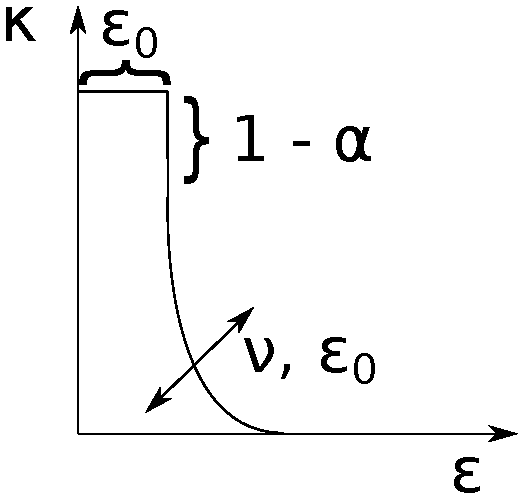
\includegraphics[height=6cm]{img/fit.pdf}
    \caption{Funkcija ovisnosti preciznosti $\kappa$ o pogrešci u predviđanju $\epsilon$. Slika preuzeta iz \citep{5}}
    \label{img:fit}
\end{figure}
Na slici \ref{img:fit} vidi se utjecaj pojedinih parametara prilikom računanja preciznosti $\kappa$.
Parametar $\epsilon_{0}$ određuje do koje granice će pravila imati jednaku, maksimalnu, preciznost, parametar $\alpha$ uvodi značajnu razliku između preciznih i manje preciznih pravila, a parametri $\nu$ i ponovno $\epsilon_{0}$ određuju brzinu opadanja preciznosti.

Nakon postavljanja parametara, postoji mogućnost za pokretanjem operacije istraživanja novih pravila \engl{discovery component}.
Svako pravilo dodatno sadrži i parametar koji pamti kada je zadnji put ono sudjelovao u akcijskom setu nad kojim se provela operacija istraživanja novih pravila.
Operacija otkrivanja novih pravila provodi se ukoliko je prosječno vrijeme proteklo od prošlog pokretanja operacije otkrivanja nad pravilima unutar akcijskog skupa veće od vremena određenog konstantom $\theta_{GA}$.
Ukoliko to nije zadovoljeno, ovaj se korak preskače.

Prilikom operacije otkrivanja, najprije se iz akcijskog skupa izabiru dva roditeljska pravila.
Odabir roditeljskih pravila ostvaren je turnirskom selekcijom \engl{tournament selection} u ovisnosti o parametru dobrote.
Prilikom turnirske selekcije, nasumično se odabire unaprijed zadani broj pravila, te se kao pobjednika odabire onaj koji od odabranih ima najveću vrijednost dobrote.
Od izabranih roditeljskih pravila stvaraju se dva potomka, od kojih prvotno svaki ima iste programske isječke uvjeta kao jedan od roditelja.

Nakon toga, s vjerojatnošću $\chi$ provodi se križanje potomaka.
Križanje je ostvarenom operacijom križanja u dvije točke \engl{two-point crossover} kako je prikazano algoritmom \ref{alg:cross}.
\begin{algorithm}[h]
    \caption{Križanje u dvije točke}
    \label{alg:cross}
    \begin{algorithmic}
        \STATE{\textbf{Ulaz:} $cl_{1}$ -- prvo pravilo, $cl_{2}$ -- drugo pravilo.}
        \STATE{\textbf{Izlaz:} -}
        \STATE{$x :=$ proizvoljan decimalni broj iz intervala [0, n)}
        \STATE{$y :=$ proizvoljan decimalni broj iz intervala [0, n)}
        \IF{$x > y$}
        \STATE{zamijeni $x$ i $y$}
        \ENDIF
        \FOR{$(i = x; i <= y; i = i + 1)$}
        \STATE{zamijeni $cl_{1}.cond[i]$ i $cl_{2}.cond[i]$}
        \ENDFOR
    \end{algorithmic}
\end{algorithm}
Prilikom križanja u dvije točke, proizvoljno se odabiru dva mjesta unutar uvjeta pravila koja se križaju, te se zamjene svi programski isječci između njih.
Unutar algoritma, varijabla $n$ sadrži duljinu uvjeta, odnosno broj programskih isječaka.
Programski isječci se ovdje ne mijenjaju, samo se razmjenjuju između potomaka.
Također, prilikom operacije križanja, akcije koje pravila zagovaraju se ne mijenjaju.

Nakon toga, nad potomcima se provodi mutacija, u kojoj svaki programski isječak uvjeta ima vjerojatnost mutacije $\mu$.
Mutacija, za razliku od križanja, djeluje i na uvjete pravila i na akcije.
Tijekom mutacije, svaki simbol \emph{don't care} zamjenjuje se proizvoljno generiranim programskim isječkom koji odgovara stanju $s$ dobivenom iz okoline, a svaki drugi programski isječak zamjenjuje se simbolom \emph{don't care}.
Na poslijetku, akcije potomaka također bivaju mutirane s vjerojatnošću $\mu$, pri čemu se akcija mijenja u bilo koju drugu akciju (u ovom radu su jedine moguće akcije 0 ili 1, stoga 0 postaje 1, a 1 postaje 0).
Nakon mutacije, mutirani potomak još uvijek odgovara stanju $s$.
Operacija mutacije prikazana je algoritmom \ref{alg:mut}
\begin{algorithm}[h]
    \caption{Mutacija}
    \label{alg:mut}
    \begin{algorithmic}
        \STATE{\textbf{Ulaz:} $cl$ -- klasifikator nad kojim se provodi mutacija, $s$ -- stanje okoline.}
        \STATE{\textbf{Izlaz:} -}
        \FOR{$(i = 1; i <= n; i = i + 1)$}
        \STATE{$r :=$ proizvoljan decimalni broj iz intervala [0, 1)}
        \IF{$r < \mu$}
        \IF{$cl.cond[i] =$ \emph{don't care} simbol}
        \REPEAT
        \STATE{$cf$ := generiraj proizvoljni programski isječak}
        \STATE{$val := evaluiraj(cf, s)$}
        \UNTIL{$val \neq 1$}
        \STATE{$cl.cond[i] := cf$}
        \ELSE
        \STATE{$cl.cond[i]$ := \emph{don't care} simbol}
        \ENDIF
        \ENDIF
        \ENDFOR
        \STATE{$r :=$ proizvoljan decimalni broj iz intervala [0, 1)}
        \IF{$r < \mu$}
        \STATE{$cl.action :=$ proizvoljna akcija različita od $cl.action$}
        \ENDIF
    \end{algorithmic}
\end{algorithm}

Na kraju operacije istraživanja, predviđanje novonastalih potomaka postavlja se na srednju vrijednost predviđanja roditelja, pogreška u predviđanju postavlja se na srednju vrijednost pogreške u predviđanju roditelja pomnoženu faktorom $predictionErrorReduction$, a dobrota na srednju vrijednost dobrote roditelja pomnoženu faktorom $fitnessReduction$, kao što je navedeno u \citep{4}.

Prije dodavanja nastalih potomaka u populaciju, pokreće se operacija provjere obuhvaća li neki od roditelja potomke \engl{GA subsumption}.
Roditelj obuhvaća potomka, ako uvjet roditelja logički obuhvaća uvjet potomka.
Razlog ovoj operaciji je taj što u slučaju da roditelj obuhvaća potomka, dodavanjem potomka u populaciju ne bi se poboljšala sposobnost sustava, jer roditelj sadrži sve informacije koje sadrži i potomak \citep{1}.
Da bi se uopće mogla pokrenuti provjera, roditelj mora biti precizan i dovoljno iskusan.
Konstanta $\theta_{sub}$ sadrži donju granicu iskustva pravila da bi se za njega moglo reći da je dovoljno iskusno za ovu operaciju, dok konstanta $\epsilon_{0}$ sadrži gornju granicu pogreške u predviđanju pravila da bi oni bilo dovoljno precizno.
Roditelj može obuhvatiti potomka ako oba pravila zagovaraju istu akciju, ako je roditelj precizan i dovoljno iskusan i ako je roditelj općenitiji od potomka.
Uvođenjem programskih isječaka umjesto simbola ternarne abecede u uvjete pravila, maknuta je važnost poretka programskih isječaka unutar uvjeta.
Iz tog razloga, prilikom ispitivanja je li roditelj općenitiji od djeteta u obzir su uzeti skupovi programskih odsječaka \citep{4}.
Operacija provjere je li jedno pravilo općenitije od drugog prikazana je algoritmom \ref{alg:general}
\begin{algorithm}
    \caption{Općenitije pravilo}
    \label{alg:general}
    \begin{algorithmic}
        \STATE{\textbf{Ulaz:} $cl_{1}$ -- općenitije pravilo, $cl_{2}$ -- specifičnije pravilo.}
        \STATE{\textbf{Izlaz:} -- je li pravilo $cl_{1}$ općenitije od $cl_{2}$}
        \STATE{$x :=$ broj \emph{don't care} simbola u $cl_{1}$}
        \STATE{$y :=$ broj \emph{don't care} simbola u $cl_{2}$}
        \IF{$x \leq y$}
        \RETURN{$false$}
        \ENDIF
        \STATE{$X :=$ skup svih "ne-\emph{don't care}" isječaka u $cl_{1}$}
        \STATE{$Y :=$ skup svih "ne-\emph{don't care}" isječaka u $cl_{2}$}
        \IF{$X \not \subseteq Y$}
        \RETURN{$false$}
        \ENDIF
        \RETURN{$true$}
    \end{algorithmic}
\end{algorithm}
Da bi pravilo $cl_{1}$ bilo općenitije od pravila $cl_{2}$, $cl_{1}$ mora imati više simbola \emph{don't care} od pravila $cl_{2}$, a svaki ostali programski isječak pravila $cl_{1}$ mora biti sadržan u $cl_{2}$.
Ako se pokaže da roditelj obuhvaća potomka, umjesto dodavanja tog potomka u populaciju, roditelju se parametar brojnosti povećava za 1.

Nakon provjere obuhvaća li roditelj potomka, pokreće se provjera obuhvaćanja unutar cijelog akcijskog skupa [\emph{A}].
Pretražuje se akcijski skup i pronalazi se pravilo koje je precizno i dovoljno iskusno, a ima najveći udio simbola \emph{don't care}.
Da bi pravilo bilo precizno i dovoljno iskusno za obuhvaćanje drugih pravila, ono mora ispunjavati isti uvjet kao i u prethodnom koraku.
Nakon pronalaženja takvog pravila $cl$, ponovno se prolazi kroz akcijski skup i za svako pravilo $c$ od kojega je $cl$ općenitije, pravilu $cl$ se brojnost povećava za brojnost pravila $c$, a klasifikator $c$ se briše iz populacije.

Nadalje, prilikom dodavanja novog pravila $cl$ u populaciju, potrebno je proći kroz ostala pravila u populaciji i provjeriti postoji li već pravilo koje je jednako pravilu $cl$.
Ako takvo pravilo postoji, $cl$ se ne dodaje u populaciju, nego se pronađenom pravilu brojnost poveća za 1.
Postupak provjere jednakosti pravila također je drugačiji u odnosu na klasični sustav XCS.
Ponovno nije bitno da poredak programskih isječaka u pravilima bude jednak, nego da pravila sadrže jednake isječke, neovisno o poziciji.
Postupak provjere jednakosti pravila prikazan je algoritmom \ref{alg:eq}.
\begin{algorithm}
    \caption{Jednakost pravila}
    \label{alg:eq}
    \begin{algorithmic}
        \STATE{\textbf{Ulaz:} $cl_{1}$ -- prvo pravilo, $cl_{2}$ -- drugo pravilo.}
        \STATE{\textbf{Izlaz:} -- je li pravilo $cl_{1}$ općenitije od $cl_{2}$}
        \IF{$cl_{1}.action \neq cl_{2}.action$}
        \RETURN{$false$}
        \ENDIF
        \STATE{$x :=$ broj simbola \emph{don't care} u $cl_{1}$}
        \STATE{$y :=$ broj simbola \emph{don't care} u $cl_{2}$}
        \IF{$x \neq y$}
        \RETURN{$false$}
        \ENDIF
        \STATE{$X :=$ skup svih "ne-\emph{don't care}" isječaka u $cl_{1}$}
        \STATE{$Y :=$ skup svih "ne-\emph{don't care}" isječaka u $cl_{2}$}
        \IF{$X \neq Y$}
        \RETURN{$false$}
        \ENDIF
        \RETURN{$true$}
    \end{algorithmic}
\end{algorithm}
Da bi pravila bila jednaka, ona moraju zagovarati istu akciju, moraju imati jednak broj simbola \emph{don't care}, a skupovi ostalih programskih isječaka tih pravila moraju biti jednaki.

Prilikom generiranja proizvoljnih programskih isječaka, kao listovi unutar binarnog stabla, osim terminalnih čvorova, koriste se i programski isječci naučeni na jednostavnijim problemima unutar iste domene \citep{4}.
Po završetku učenja određenog problema, sakupljeni su programski isječci sadržani unutar preciznih i iskusnih pravila konačne populacije.
Pravilo je precizno i dovoljno iskusno za korištenje pri učenju težeg problema ako je njegovo iskustvo veće od konstante $\theta_{re}$ i ako je njegova dobrota veća od prosječne dobrote konačne populacije.
Primjer ponovnog korištenja naučenih programskih isječaka prikazan je u tablici \ref{tbl:reuse}.
U tablici je različitim programskim isječcima dano ime zbog jednostavnijeg referenciranja.
Vidi se da su isječci naučeni na najjednostavnijem 4/1 multipleksoru korišteni kao listovi unutar isječaka 8/1 multipleksora.
Jednako tako, u 16/1 multipleksoru, korišteni su isječci naučeni i na 4/1 i 8/1 multipleksoru.
\begin{table}[!htb]
    \caption{Ponovno korištenje naučenog znanja. Tablica preuzeta iz \citep{4}.}
    \label{tbl:reuse}
    \centering
    \begin{tabular}{c | c | c}
        \multirow{2}{*}{Multipleksor} & \multicolumn{2}{c}{Programski isječak} \\
        & Ime & Izraz \\ \hline
        \multirow{3}{*}{MUX 4/1} & L1\_0 & $D_{1}D_{0}D_{4}dr$ \\
        & L1\_1 & $D_{5}\sim D_{1}D_{0}\&\&$ \\
        & ... & ... \\ \hline
        \multirow{3}{*}{MUX 8/1} & L2\_0 & $L1\_15D_{2}L1\_4r\&$ \\
        & L2\_1 & $L1\_5D_{7}|L1\_11D_{3}\&r$ \\
        & ... & ... \\ \hline
        \multirow{3}{*}{MUX 16/1} & L3\_0 & $L2\_9L1\_7D_{11}|r$ \\
        & L3\_1 & $L1\_10D_{17}|L2\_1D_{0}r\&$ \\
        & ... & ... \\
    \end{tabular}
\end{table}

U načinu rada \emph{iskoristi}, sustav XCS se ne mijenja, nego izvršava najbolju moguću akciju.
Početak je isti kao i u načinu rada \emph{istraži}.
Formira se podudarni skup koji se sastoji od pravila koja odgovaraju ulazu $s$.
U ovisnosti o pravilima sadržanim u [\emph{M}], formira se \emph{polje predviđanja}, na isti način kako je opisano u načinu rada \emph{istraži}.
Na temelju formiranog \emph{polja predviđanja}, odabire se akcija $a$ s najvećom vrijednosti $P(a)$.
Ovaj odabir je drugačiji od onog opisanog u načinu rada \emph{istraži}, u kojem se akcija $a$ odabire \emph{Roulette-Wheel} postupkom u ovisnosti o vrijednosti $P(a)$.

Načini rada \emph{istraži} i \emph{iskoristi} se međusobno izmjenju, pri čemu način rada \emph{iskoristi} služi testiranju sposobnosti sustava.

\chapter{Rezultati} \label{ch:res}
Prilikom testiranja rada sustava, korištene vrijednosti parametara sustava su podešene kao u \citep{4}.
Stopa učenja $\beta = 0.2$, stopa propadanja dobrote $\alpha = 0.1$, granica pogreške predviđanja $\epsilon_{0} = 10$, eksponent propadanja dobrote $\nu = 5$, granica prosječnog proteklog vremena prilikom istraživanja novih pravila $\theta_{GA} = 25$, vjerojatnost križanja u dvije točke $\chi = 0.8$, vjerojatnost mutacije $\mu$, granica iskustva pri brisanju pravila $\theta_{del} = 20$, postotak srednje vrijednosti dobrote prilikom brisanja $\delta = 0.1$, granica iskustva prilikom obuhvaćanja $\theta_{sub} = 20$, vjerojatnost pojavljivanja simbola \emph{don't care} $P_{don'tCare} = 0.33$, propadanje pogreške predviđanja $predictionErrorReduction = 0.25$, propadanje dobrote $fitnessReduction = 0.1$.
Veličina turnira prilikom turnirske selekcije je $40\%$ veličine akcijskog skupa.
Nagrada okoline iznosi 1000 za ispravnu klasifikaciju, a 0 za neispravnu.
Prilikom generiranja novih programskih isječaka, terminalni čvor ima 50\% vjerojatnosti poprimanja programskog isječka naučenog na nižim razinama.
Na osi apscisa nalazi se broj do tad korištenih testnih primjera, a na osi ordinata pomični udio točno klasificiranih primjera prilikom prethodnih 1000 iteracija \emph{iskoristi}.

Sva testiranja odrađena su na AMD A10-8700p četverojezgrenom procesoru frekvencije 1.8 GHz i radnoj memoriji od 12 GB.

\begin{figure}[!h]
    \centering
    \begin{subfigure}{0.496\textwidth}
        \centering
        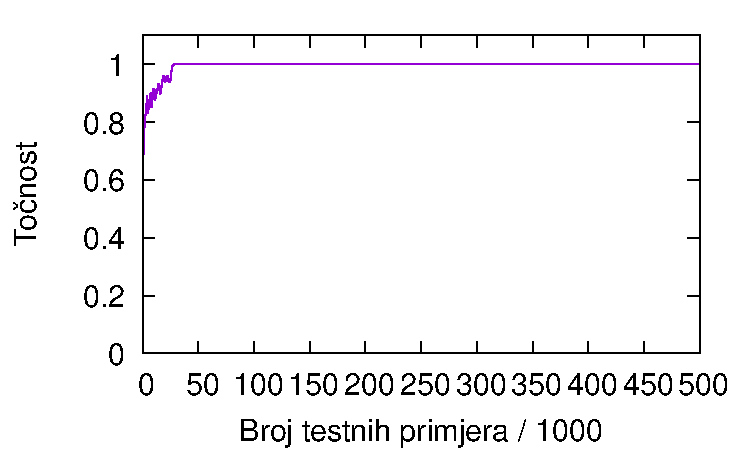
\includegraphics[width=\textwidth]{img/multiplexer/6muxre.pdf}
        \caption{4/1 multipleksor.}
        \label{fig:6muxre}
    \end{subfigure}
    %\hspace{0.05\textwidth}
    \begin{subfigure}{0.496\textwidth}
        \centering
        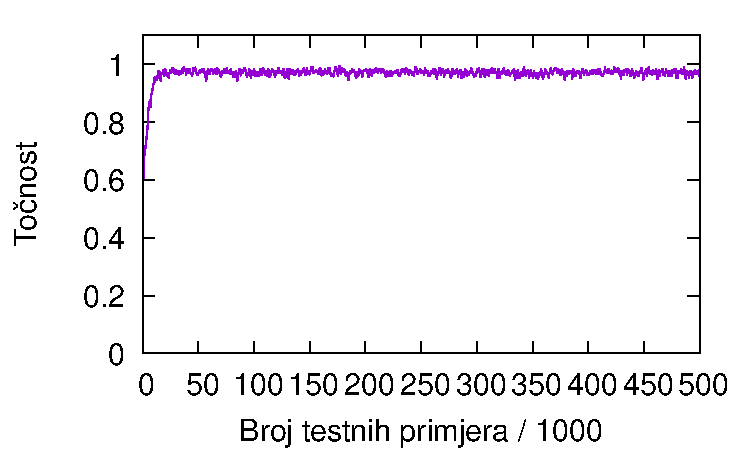
\includegraphics[width=\textwidth]{img/multiplexer/11muxre.pdf}
        \caption{8/1 multipleksor.}
        \label{fig:11muxre}
    \end{subfigure}
    \begin{subfigure}{0.496\textwidth}
        \centering
        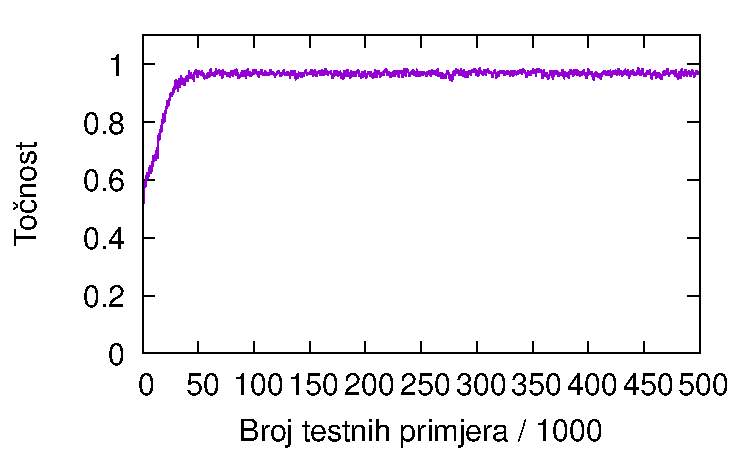
\includegraphics[width=\textwidth]{img/multiplexer/20muxre.pdf}
        \caption{16/1 multipleksor.}
        \label{fig:20muxre}
    \end{subfigure}
    %\hspace{0.05\textwidth}
    \begin{subfigure}{0.496\textwidth}
        \centering
        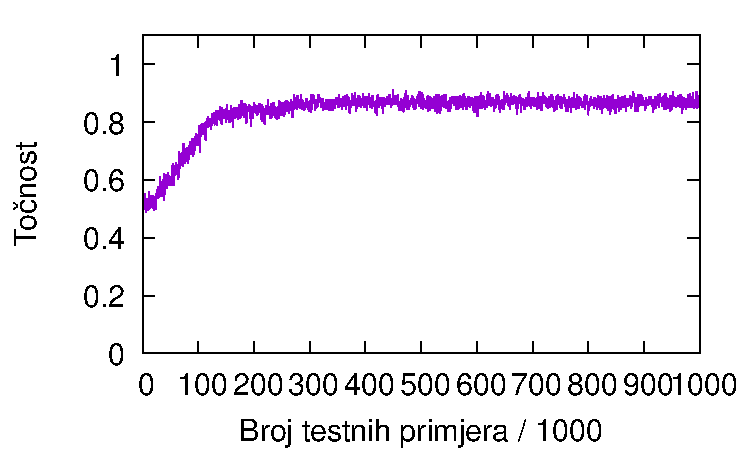
\includegraphics[width=\textwidth]{img/multiplexer/37muxre.pdf}
        \caption{32/1 multipleksor.}
        \label{fig:37muxre}
    \end{subfigure}
    \caption{Ponašanje sustava na problemu multipleksora s iskorištavanjem već naučenog znanja.}
    \label{fig:muxre}
\end{figure}
Na slici \ref{fig:muxre} prikazani su grafovi ponašanja sustava na problemu multipleksora.
Veličina populacije $N$ redom je 500, 1000, 2000, 5000 za 4/1, 8/1, 16/1 odnosno 32/1 multipleksor.
4/1, 8/1 i 16/1 multipleksori trenirani su na $5 \cdot 10^{5}$ testnih primjera, a 32/1 na $10^{6}$.
Treniranje za 4/1, 8/1 i 16/1 multipleksor trajalo je ukupno oko 7 minuta, dok je treniranje 32/1 multipleksora trajalo otprilike 50 minuta.
Broj mogućih različitih primjera 32/1 multipleksora je $2^{37} \approx 10^{11}$.
Iz slike \ref{fig:37muxre} se vidi da je već nakon otprilike $3 \cdot 10^{5}$ testnih primjera točnost sustava oko 90\% iako je prostor pretraživanja jako velik, XCSCFC se na njemu ponaša poprilično dobro.

\begin{figure}[!h]
    \centering
    \begin{subfigure}{0.496\textwidth}
        \centering
        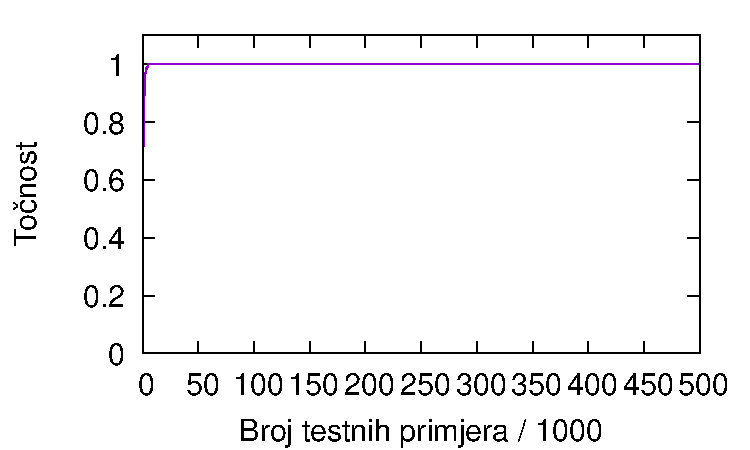
\includegraphics[width=\textwidth]{img/multiplexer/6muxnre.pdf}
        \caption{4/1 multipleksor.}
        \label{fig:6muxnre}
    \end{subfigure}
    %\hspace{0.05\textwidth}
    \begin{subfigure}{0.496\textwidth}
        \centering
        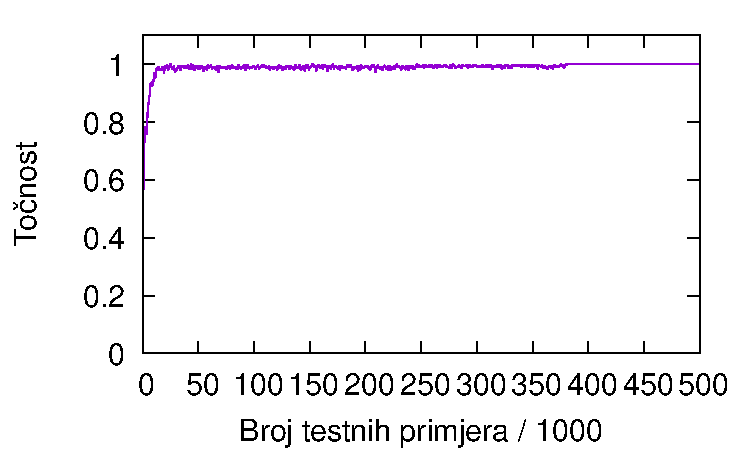
\includegraphics[width=\textwidth]{img/multiplexer/11muxnre.pdf}
        \caption{8/1 multipleksor.}
        \label{fig:11muxnre}
    \end{subfigure}
    \begin{subfigure}{0.496\textwidth}
        \centering
        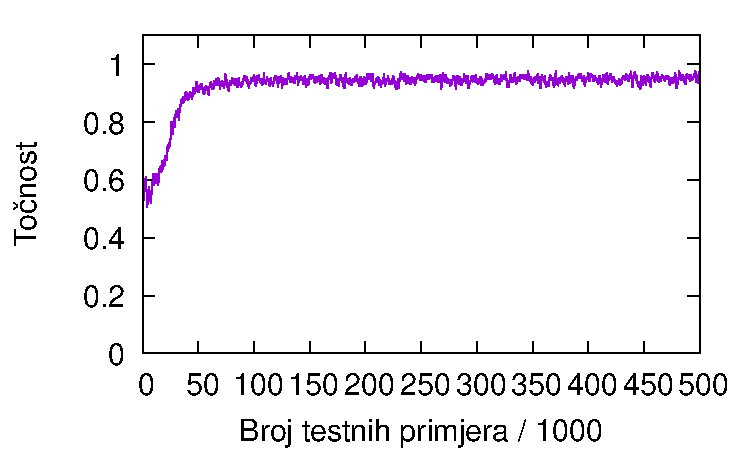
\includegraphics[width=\textwidth]{img/multiplexer/20muxnre.pdf}
        \caption{16/1 multipleksor.}
        \label{fig:20muxnre}
    \end{subfigure}
    %\hspace{0.05\textwidth}
    \begin{subfigure}{0.496\textwidth}
        \centering
        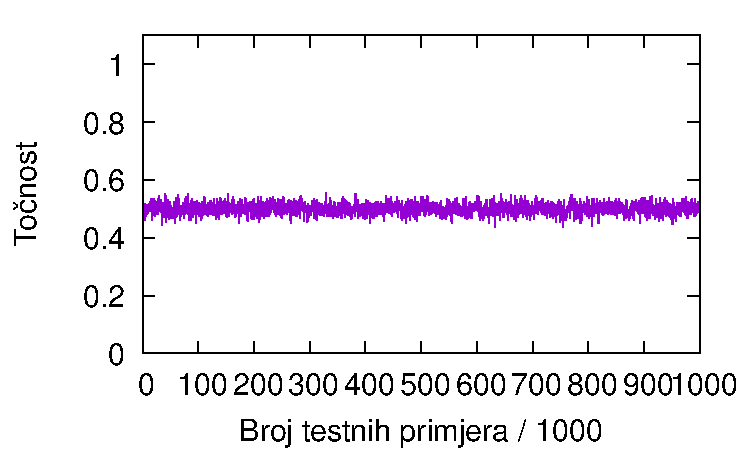
\includegraphics[width=\textwidth]{img/multiplexer/37muxnre.pdf}
        \caption{32/1 multipleksor.}
        \label{fig:37muxnre}
    \end{subfigure}
    \caption{Ponašanje sustava na problemu multipleksora bez iskorištavanja već naučenog znanja.}
    \label{fig:muxnre}
\end{figure}
S obzirom da je, izmeđuostalog, cilj rada bio prikazati kako radi ponovno iskorištavanje naučenog znanja na manjim problemima, za usporedbu, na slici \ref{fig:muxnre} prikazan je graf ponašanja sustava na problemu multipleksora, ali bez korištenja prethodno stečenog znanja.
Ovdje je svaki multipleksor učen od nule, bez znanja o manjim multipleksorima.
Posebno je zanimljivo pogledati sliku \ref{fig:37muxnre} iz koje se vidi da u ovom slučaju, na primjeru 32/1 multipleksora, sustav nije naučio gotovo ništa, nasuprot vrlo dobrom rezultatu prilikom učenja 32/1 multipleksora uz korištenje prethodno stečenog znanja.

\begin{figure}[!h]
    \centering
    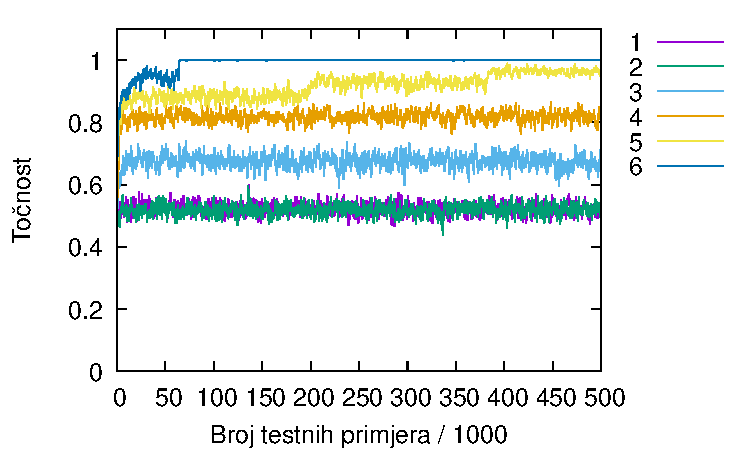
\includegraphics[width=12cm]{img/mux_cond/6bitcond.pdf}
    \caption{Prikaz učenja 6 bitnog multipleksora u ovisnosti o broju programskih isječaka koje klasifikatori sadržavaju.}
    \label{img:6bitcond}
\end{figure}
S obzirom da je, uvođenjem programskih isječaka umjesto uvjetnih bitova, maknuta ovisnost duljine ulaza dobivenog od okoline i broja uvjetnih bitova unutar pravila, prilikom korištenja XCSCFC sustava moguće je imati broj programskih isječaka različit od veličine ulaza.
U svrhu testiranja ovisnosti broja programskih isječaka unutar pojedinog pravila i kvalitete XCSCFC sustava, na slici \ref{img:6bitcond} prikazan je graf ponašanja sustava na 4/1 multipleksoru s različitim brojevima programskih isječaka.
Rezultat je očekivan, a vidi se i da između korištenja jednog programskog isječka i korištenja dva programska isječka u ovom primjeru nema razlike.

\begin{figure}[!h]
    \centering
    \begin{subfigure}{0.496\textwidth}
        \centering
        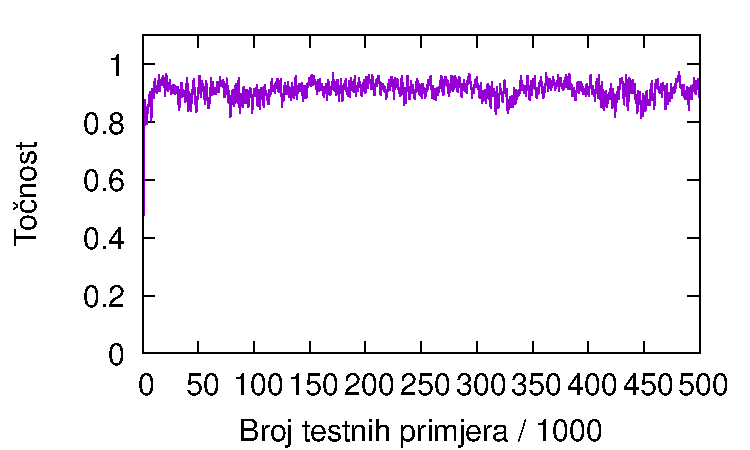
\includegraphics[width=\textwidth]{img/majority/3majre.pdf}
        \caption{Problem s 3 bita.}
        \label{fig:3majre}
    \end{subfigure}
    \begin{subfigure}{0.496\textwidth}
        \centering
        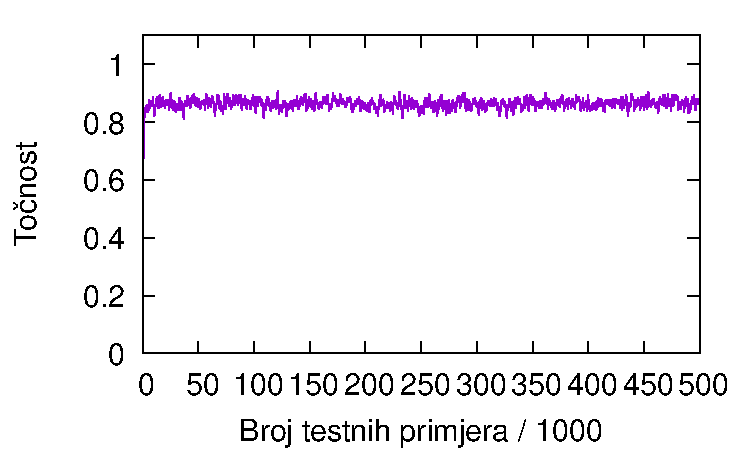
\includegraphics[width=\textwidth]{img/majority/5majre.pdf}
        \caption{Problem s 5 bita.}
        \label{fig:5majre}
    \end{subfigure}
    \begin{subfigure}{0.496\textwidth}
        \centering
        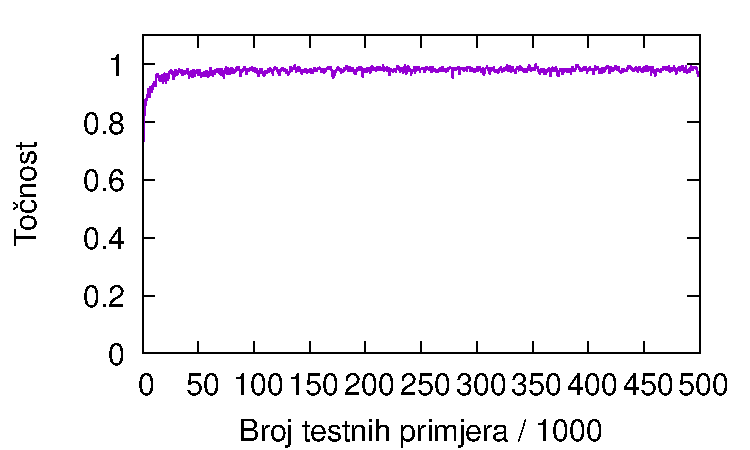
\includegraphics[width=\textwidth]{img/majority/7majre.pdf}
        \caption{Problem sa 7 bita.}
        \label{fig:7majre}
    \end{subfigure}
    \caption{Ponašanje sustava na problemu pronalaska bita s najvećom frekvencijom pojavljivanja.}
    \label{fig:majre}
\end{figure}
Rezultati dobiveni na problemu najzastupljenijeg bita prikazani su na slici \ref{fig:majre}.
Veličina populacije $N$ ovdje je redom 500, 1000 i 2000 za 3-, 5- i 7-bitni problem.
Broj testnih primjera za svaku veličinu je $5 \cdot 10^{5}$.
Prostor pretraživanja je ovdje znatno manji od onoga u problemu s multipleksorom, rezultati nisu znatno bolji.
Zanimljivo je primjetiti da je sustav ovdje bolje naučio 7-bitni (slika \ref{fig:7majre}) problem nego 3-bitni (slika \ref{fig:3majre}), a prostor pretraživanja u 7-bitnom problemu je 16 puta veći.

\begin{figure}[!h]
    \centering
    \begin{subfigure}{0.496\textwidth}
        \centering
        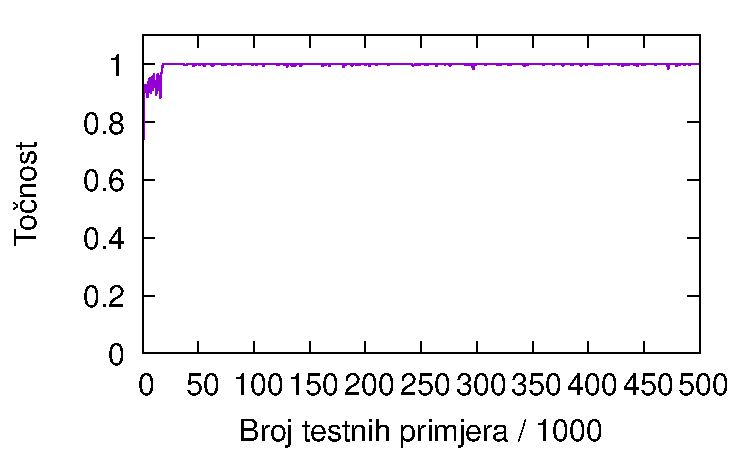
\includegraphics[width=\textwidth]{img/parity/2pare.pdf}
        \caption{Problem s 2 bita.}
        \label{fig:2pare}
    \end{subfigure}
    \begin{subfigure}{0.496\textwidth}
        \centering
        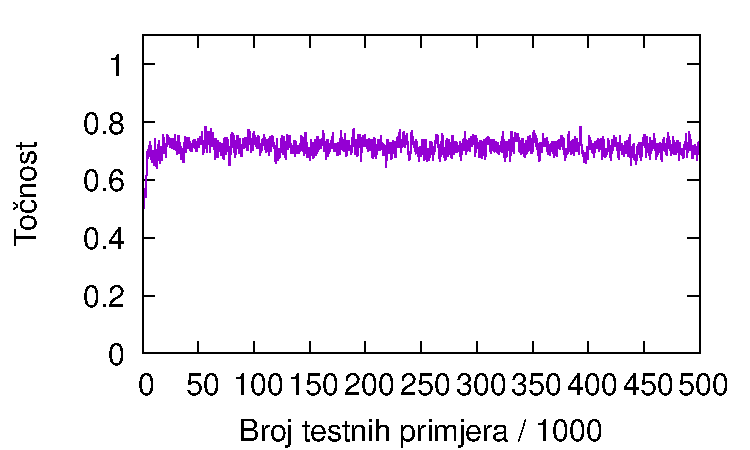
\includegraphics[width=\textwidth]{img/parity/3pare.pdf}
        \caption{Problem s 3 bita.}
        \label{fig:3pare}
    \end{subfigure}
    \begin{subfigure}{0.496\textwidth}
        \centering
        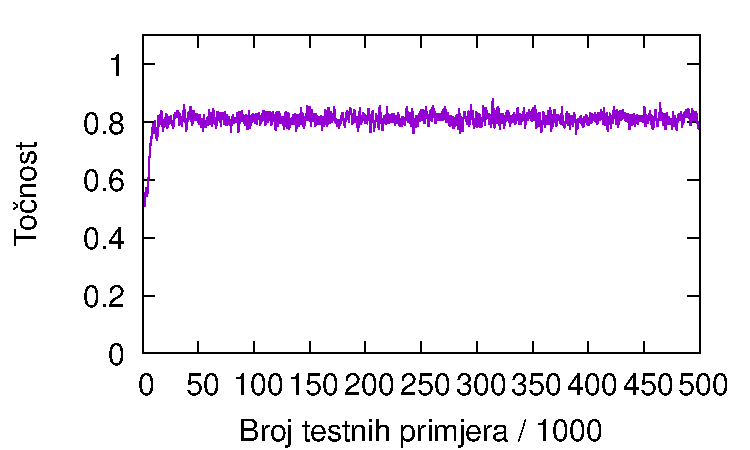
\includegraphics[width=\textwidth]{img/parity/4pare.pdf}
        \caption{Problem s 4 bita.}
        \label{fig:4pare}
    \end{subfigure}
    \begin{subfigure}{0.496\textwidth}
        \centering
        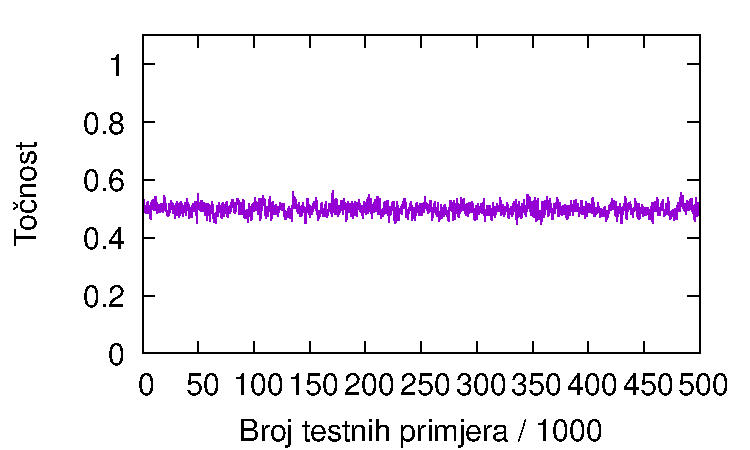
\includegraphics[width=\textwidth]{img/parity/5pare.pdf}
        \caption{Problem s 5 bita.}
        \label{fig:5pare}
    \end{subfigure}
    \caption{Ponašanje sustava na problemu parnog pariteta.}
    \label{fig:pare}
\end{figure}
Rezultati na problemu parnog pariteta prikazani su na slici \ref{fig:pare}.
Veličina populacije $N$ redom je 200, 300, 400, 500 za 2-, 3-, 4- i 5-bitni problem.
Broj testnih primjera za svaku veličinu je $5 \cdot 10^{5}$.
Iz slike se vidi da je problem s 2 bita (slika \ref{fig:2pare}) riješen s jako velikom točnošću, ali zbog toga što je vjerojatno naučen na pamet.
Iz slike \ref{fig:3pare} se vidi da se već prilikom učenja za 3 bita javljaju problemi.
Na problemu s 5 bita (\ref{fig:5pare}) sustav nije uspio ništa generalizirati i rezultat je gotovo proizvoljan.

\begin{figure}[!h]
    \centering
    \begin{subfigure}{0.496\textwidth}
        \centering
        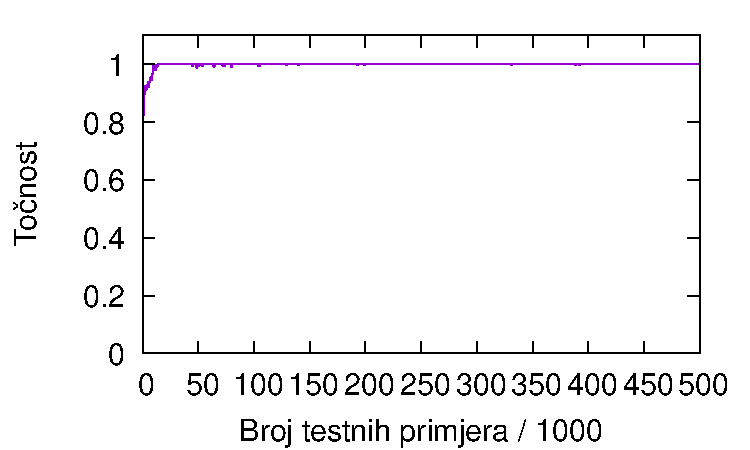
\includegraphics[width=\textwidth]{img/carry/4care.pdf}
        \caption{Zbrajanje 2-bitnih brojeva.}
        \label{fig:4care}
    \end{subfigure}
    \begin{subfigure}{0.496\textwidth}
        \centering
        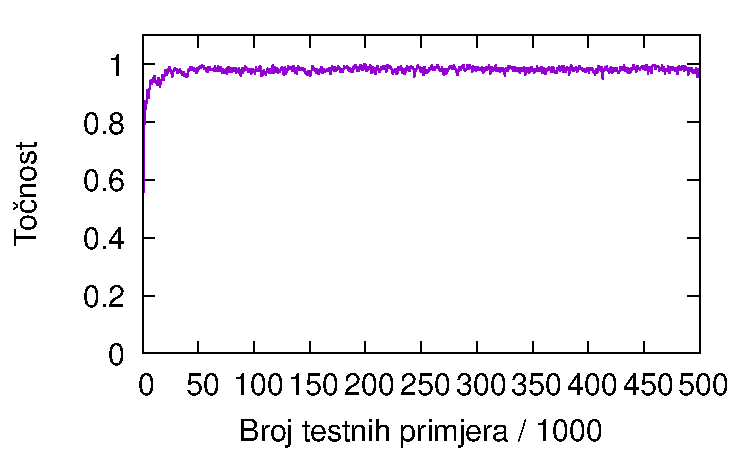
\includegraphics[width=\textwidth]{img/carry/6care.pdf}
        \caption{Zbrajanje 3-bitnih brojeva.}
        \label{fig:6care}
    \end{subfigure}
    \begin{subfigure}{0.496\textwidth}
        \centering
        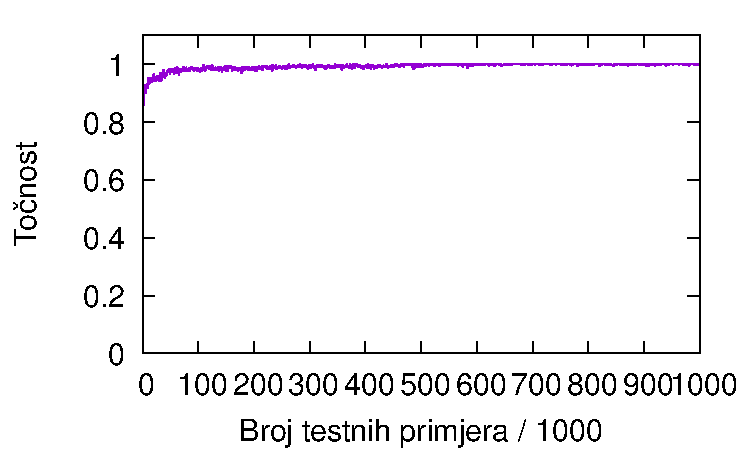
\includegraphics[width=\textwidth]{img/carry/8care.pdf}
        \caption{Zbrajanje 4-bitnih brojeva.}
        \label{fig:8care}
    \end{subfigure}
    \begin{subfigure}{0.496\textwidth}
        \centering
        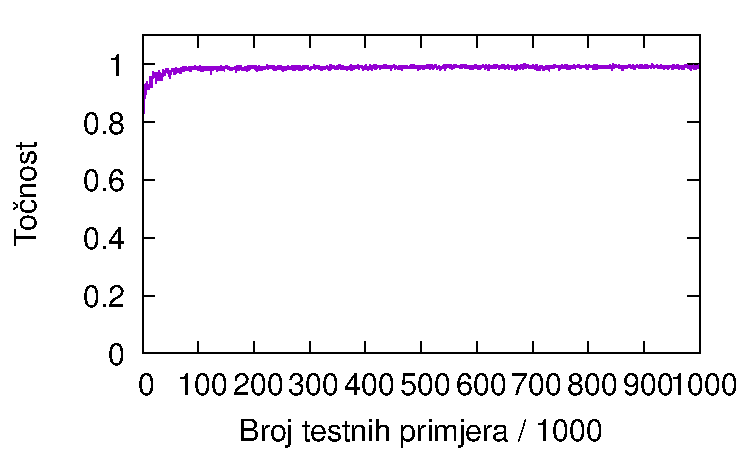
\includegraphics[width=\textwidth]{img/carry/10care.pdf}
        \caption{Zbrajanje 5-bitnih brojeva.}
        \label{fig:10care}
    \end{subfigure}
    \caption{Ponašanje sustava na problemu bita prijenosa prilikom binarnog zbrajanja.}
    \label{fig:care}
\end{figure}
Rezultati na problemu određivanja bita prijenosa prilikom zbrajanja binarnih brojeva prikazani su grafom na slici \ref{fig:care}.

\chapter{Zaključak} \label{ch:zak}
Susta XCS pokazao se kao vrlo složen, koji za neke probleme (npr. multipleksor) radi iznimno dobro, a za neke (npr. paritet) poprilično loše.

Zbog podjele sustava u više dijelova koji slijedno djeluju, otvara se puno prostora za isprobavanje.
Sustav ima brojne parametre s kojima se može eksperimentirati i prilagoditi ga problemu koji se rješava.

U okviru ovog rada isproban je rad sustava samo na booleovim funkcijama, ali one predstavljaju temelj za nastavak rada na složenijim problemima.
Budući rad na ovom sustavu može uključivati prilagodbu sustava za klasifikaciju (npr. jednostavnih slika) u više razreda.

Ovaj rad je motiviran radom prikazanim u \citep{4}, no ovdje su rezultati nešto lošiji nego što je prikazano u navedenom radu.
Razlog je najvjerojatnije taj što neki dijelovi nisu precizno objašnjeni, ali glavna poanta rada je usvojena.

Na primjeru multipleksora pokazano je da korištenje znanja prethodno naučenog na jednostavnijim primjerima unutar iste domene poboljšava rezultate sustava.
Znanje s nižih razina uspješno je sakupljeno i proslijeđeno prilikom učenja na težim problemima u domeni.

\bibliography{literatura}
\bibliographystyle{fer}

\begin{sazetak}
Za rješavanje problema sa jako velikim prostorom pretraživanja potrebno je pronaći novo, drugačije rješenje, zbog trenutne velike vremenske i prostorne složenosti.
U ovom radu, ostvareno je sakupljanje znanja sa jednostavnijih problema te njihovo ponovno korištenje u složenijim problemima.
Navedena funkcionalnost ostvarena je korištenjem sustava LCS.
Sustav je testiran na problemima multipleksora, većinskog bita, bita prijenosa i parnog pariteta.
Pokazano je da sustav koristeći prethodno znanje probleme rješava bolje nego učenjem novih problema ispočetka.

\kljucnerijeci{Učeni klasifikacijski sustavi, strojno učenje, podržano učenje, genetski algoritmi, ponovno iskorištavanje znanja.}
\end{sazetak}

\engtitle{Application of LCS on Classification Problems}
\begin{abstract}
To succesfully solve a large-scale problems there has been a need for a new, different approach, due to the large time and space complexity.
In this work, knowledge extraction from smaller problems and its reuse in more complex problems has been achieved.
The proposed functionality has been achived on the LCS system.
The system is tested on multiplexer problems, majority-on problems, carry problems and even-parity problems.
It is shown that better results are achived while using the extracted knowledge than when every problem is learned from scratch.


\keywords{Learning classifier systems, machine learning, reinforcement learning, genetic algorithms, knowledge reuse.}
\end{abstract}

\end{document}

